\documentclass[a4paper,11pt]{article}

\usepackage[a4paper,margin=2.55cm]{geometry}
\usepackage{fontspec}
\usepackage{amsmath,amssymb,amsthm}
\usepackage{booktabs}
\usepackage{array}
\usepackage{enumitem}
\usepackage{xcolor}
\usepackage{hyperref}
\usepackage{listings}
\usepackage{float}
\usepackage{tikz}
\usetikzlibrary{arrows.meta,positioning,fit,shapes.geometric,decorations.pathreplacing,calc}

%% Global arrow grammar for all Morph diagrams
%% Solid  = state/value progression
%% Dashed = dependency/reference
%% Every dashed arrow must carry a semantic label
\tikzset{
  morpharrow/.style={-{Latex[length=2.1mm,width=1.5mm]}, semithick,
    draw=gray!75!black, line cap=round, shorten >=2pt, shorten <=2pt},
  morphdash/.style={morpharrow, dashed, dash pattern=on 3pt off 2pt},
  arrowlabel/.style={font=\scriptsize, fill=white, inner sep=1.3pt}
}

\setmainfont{Times}
\setsansfont{Helvetica}
\setmonofont{Menlo}[Scale=0.88]
\emergencystretch=2em
\setlength{\textfloatsep}{10pt plus 2pt minus 2pt}
\setlength{\floatsep}{8pt plus 2pt minus 2pt}
\setlength{\intextsep}{8pt plus 2pt minus 2pt}

\definecolor{MorphBlue}{HTML}{1F4E79}
\definecolor{MorphGreen}{HTML}{2F7D5A}
\definecolor{MorphAmber}{HTML}{B36B00}
\newcolumntype{L}[1]{>{\raggedright\arraybackslash}p{#1}}

\renewcommand{\abstractname}{Abstract}
\renewcommand{\contentsname}{Contents}
\renewcommand{\figurename}{Figure}
\renewcommand{\tablename}{Table}
\renewcommand{\refname}{References}

\hypersetup{
  colorlinks=true,
  linkcolor=blue!55!black,
  citecolor=blue!55!black,
  urlcolor=blue!55!black,
  pdftitle={Morph Channel: A Cell-Native Protocol Construction for Sponsored State Evidence and Local Channel Factories on CKB},
  pdfauthor={Arthur Zhang}
}

\lstdefinestyle{morph}{
  basicstyle=\ttfamily\small,
  breaklines=true,
  frame=single,
  columns=fullflexible,
  backgroundcolor=\color{gray!4},
  rulecolor=\color{gray!35}
}
\lstset{style=morph}

\newtheorem{definition}{Definition}
\newtheorem{assumption}{Assumption}
\newtheorem{invariant}{Invariant}
\newtheorem{lemma}{Lemma}
\newtheorem{proposition}{Proposition}
\newtheorem{corollary}{Corollary}
\newtheorem{remark}{Remark}

\newcommand{\Cells}{\mathcal{U}}
\newcommand{\Tx}{\mathsf{Tx}}
\newcommand{\Fund}{\mathsf{Fund}}
\newcommand{\Vault}{\mathsf{Vault}}
\newcommand{\State}{\mathsf{State}}
\newcommand{\Sponsor}{\mathsf{Sponsor}}
\newcommand{\Header}{\mathsf{Header}}
\newcommand{\Payload}{\mathsf{Payload}}
\newcommand{\Desc}{\mathsf{Desc}}
\newcommand{\Since}{\mathsf{since}}
\newcommand{\hash}{\mathsf{H}}
\newcommand{\sig}{\mathsf{Sig}}

\title{\textbf{Morph Channel}\\
\large A Cell-Native Protocol Construction for Sponsored State Evidence and Local Channel Factories on CKB}
\author{Arthur Zhang}
\date{June 2026}

\begin{document}

\begin{titlepage}
\centering
\vspace*{1.1cm}
{\sffamily\bfseries\LARGE Morph Channel\par}
\vspace{0.35cm}
{\sffamily\large A Cell-Native Protocol Construction for Sponsored State Evidence and Local Channel Factories on CKB\par}
\vspace{1.35cm}
{\normalsize Arthur Zhang\par}
\vspace{0.20cm}
{\normalsize June 2026\par}
\vspace{1.3cm}

\begin{abstract}
\noindent
CKB's Cell model allows a channel to separate the object that holds value from the object that carries dispute evidence. Morph Channel uses this separation to keep the funding identity stable whilst unilateral disputes advance a State Cell containing signed state evidence. Publication transactions are met from sponsor-owned Cells, so channel reserve, business CKB, and xUDT balances remain outside the fee ledger.

\medskip
\noindent
The construction defines a State Header signing domain that binds chain context, channel identity, funding epoch, funding anchor, vault-set commitment, state number, asset registry, settlement descriptor, and challenge policy, whilst leaving sponsor coin selection unsigned. State Cell, vault-lock, and sponsor-budget validation are specified as script-level predicates for the conservative publication, supersession, finalisation, splice, cooperative-close, and materialisation branches. Partition conservation checks occupied capacity, State Cell carrier capacity, channel reserve, business CKB, and each xUDT type separately, with transaction fees charged only to the sponsor partition.

\medskip
\noindent
For bilateral channels, Morph begins with plaintext witnesses so force-close transactions remain auditable. For factories, authority is commitment-based: access manifests, local proofs, touched leaves, and an outer envelope define the admissible transition before proof bytes are interpreted. Under signature unforgeability, hash collision resistance, CKB single-spend enforcement, and a challenge window that covers detection, publication, confirmation, fee bumping, and reorganisation margin, newer valid state evidence supersedes older settling evidence before finalisation. The construction is limited to current CKB primitives: Cells, lock scripts, type scripts, witnesses, \texttt{cell\_deps}, and \texttt{since}.
\end{abstract}

\vfill
\begin{flushleft}
\textbf{Keywords:} CKB, Cell model, payment channels, channel factories, sponsored fees, partition conservation, xUDT, state evidence
\end{flushleft}
\end{titlepage}

\tableofcontents
\clearpage

\section{Introduction and Motivation}

Payment channels and state channels keep frequent updates off-chain whilst preserving unilateral settlement on-chain when cooperation fails. The Lightning Network~\cite{lightning} is the canonical payment-channel construction, whilst eltoo~\cite{eltoo} isolates a replacement-based rule: during a dispute, newer mutually signed state should defeat stale evidence. Channel factories~\cite{factories} extend this idea to shared funding structures that support many off-chain relationships.

CKB exposes a different design point. A Cell has data, a lock script, an optional type script, capacity, and a stable outpoint~\cite{ckb-cell,ckb-tx}. A CKB channel can therefore make scripts recognise two different objects: a stable value anchor and a moving state-evidence Cell. This gives the design question:

\begin{quote}
What protocol structure is required so that CKB can express a channel whose funding object remains stable, while disputes move only signed state evidence?
\end{quote}

Morph Channel keeps channel value anchored in stable Cells, advances a distinct State Cell during disputes, and meets publication fees from sponsor-owned funds rather than channel-owned value. It uses the newer-state-wins principle, but implements it through CKB scripts, State Cells, relative \texttt{since}, and explicit value partitioning rather than Bitcoin-style output reshaping.

\subsection{Scope}

The paper focuses on script-level channel and factory architecture. It does not attempt to solve routing, liquidity discovery, gossip, privacy networks, watchtower markets, or factory governance. It also avoids any assumption of sub-second finality, DAG ordering, native channel transaction classes, or CKB node modification. All claims are bounded by existing CKB primitives.

The scope is the construction itself: threat model, object authority, transaction invariants, deployability, and benchmark obligations. The paper does not claim readiness for production deployment.

\subsection{Design Thesis}

The central thesis is:
\begin{quote}
\emph{A CKB channel becomes easier to audit when funding identity, state authority, and publication fee responsibility are separate protocol objects.}
\end{quote}

\begin{figure}[H]
\centering
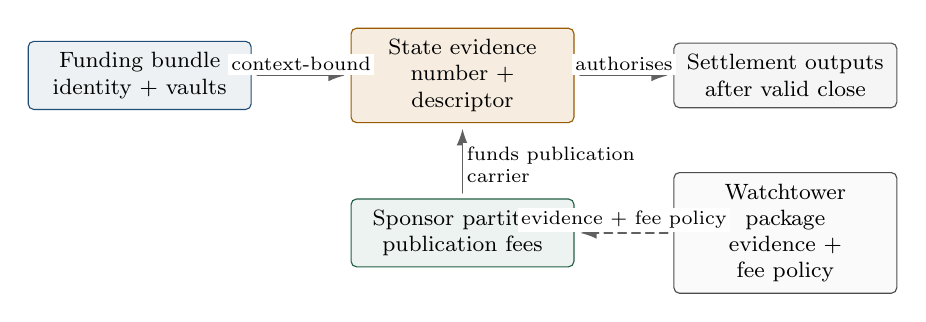
\begin{tikzpicture}[
  font=\footnotesize,
  cell/.style={draw, rounded corners=2pt, align=center, text width=2.55cm, minimum height=0.82cm, inner sep=4pt}
]
\node[cell, fill=MorphBlue!8, draw=MorphBlue] at (0,0.85) (fund) {Funding bundle\\identity + vaults};
\node[cell, fill=MorphAmber!12, draw=MorphAmber!85!black] at (4.1,0.85) (state) {State evidence\\number + descriptor};
\node[cell, fill=gray!8, draw=gray!65!black] at (8.2,0.85) (settle) {Settlement outputs\\after valid close};
\node[cell, fill=MorphGreen!9, draw=MorphGreen!75!black] at (4.1,-1.15) (sponsor) {Sponsor partition\\publication fees};
\node[cell, fill=gray!4, draw=gray!60!black] at (8.2,-1.15) (watch) {Watchtower package\\evidence + fee policy};

% State/value flow (solid)
\draw[morpharrow] (fund.east) -- node[arrowlabel, above]{context-bound} (state.west);
\draw[morpharrow] (state.east) -- node[arrowlabel, above]{authorises} (settle.west);
% Sponsor funds the carrier tx (routed with bend to avoid cramping)
\draw[morpharrow] (sponsor.north) -- node[arrowlabel, right, pos=0.45, align=left]{funds publication\\carrier} (state.south);
% Dependency/reference (dashed): watchtower supplies fee policy
\draw[morphdash] (watch.west) -- node[arrowlabel, above]{evidence + fee policy} (sponsor.east);
\end{tikzpicture}
\caption{High-level decomposition. The channel value object, the moving dispute evidence, and the fee-paying sponsor funds are separate protocol objects. Solid arrows show state/value flow; the dashed arrow shows a dependency.}
\label{fig:decomposition}
\end{figure}

Morph treats the funding object, the signed state, and the fee-paying
transaction inputs as separate authorities. The funding object identifies
channel-owned value. The State Cell and participant signatures determine how
that value may settle. Sponsor inputs fund publication without changing channel
balances. This separation keeps unilateral exit independent of wallet coin
selection and makes multi-asset conservation auditable.

\clearpage
\section{Problem Statement and Current Snapshot}

\subsection{The Funding-State Coupling Problem}

In many UTXO-oriented channel designs, settlement value and channel state are operationally coupled: a state update is represented by a new arrangement of future spend paths over the funding output. This coupling is natural in Bitcoin-like systems, but it is not inevitable on CKB. Since Cells can carry explicit typed state, a channel may maintain a stable funding anchor and move a separate state object.

If the value-holding object is also the state-update object, a force-close template can mix settlement authorisation, fee selection, and asset accounting in one place. Morph separates those checks: the vault protects channel value, the State Cell carries dispute evidence, and sponsor inputs fund the carrier transaction.

\subsection{The Fee-Boundary Problem}

A fee cap and a zero channel-paid fee policy are not equivalent. A fee cap says that channel value may be consumed up to a limit. A zero channel-paid fee invariant says that publication fees are not part of channel-owned value at all. CKB makes this distinction particularly important because capacity simultaneously represents storage resource, fee medium, and sometimes user-visible business value.

\subsection{The Authority Object Problem}

A channel protocol should not let scripts accept several competing authority sources. In a poorly separated design, authority may drift among:
\begin{enumerate}[label=(\arabic*)]
  \item the funding Cell;
  \item a plaintext witness;
  \item a local plaintext snapshot;
  \item a root commitment;
  \item a transaction body containing incidental sponsor inputs.
\end{enumerate}

Morph Channel reduces authority to a signed state header plus the admissible witness or proof required by its mode. Transaction bodies remain reconstructible wrappers around that evidence.

\clearpage
\section{Research Contributions and Design Principles}

\subsection{Main Contributions}

This paper makes nine contributions.

\begin{enumerate}[label=C\arabic*.]
  \item \textbf{Stable funding and moving evidence.} It defines a dual-track Cell construction in which channel value remains in stable funding and vault Cells, while disputes move a State Cell.
  \item \textbf{State-header-centric signing.} It specifies a canonical signing domain that binds identity and semantics while excluding sponsor coin-selection details.
  \item \textbf{Sponsored publication.} It defines a sponsor-owned publication partition and requires unilateral publication to be fee-bumpable without counterparty re-signing.
  \item \textbf{Partition conservation.} It replaces fee-cap reasoning with exact conservation of channel-owned value and fee extraction from sponsor-owned value.
  \item \textbf{Splice-aware funding identity.} It distinguishes stable logical channel identity from the current funding epoch, funding anchor, and vault set, so resizing a channel does not make stale evidence reusable.
  \item \textbf{Bilateral/factory witness separation.} It argues that bilateral channels should begin with plaintext witnesses, while factories require commitment-authoritative local proofs.
  \item \textbf{Envelope-first factory authorisation.} It separates admission of a factory transition from interpretation of its proof body: a bounded outer claim names the transition family and commits to one evidence body.
  \item \textbf{Challenge-window budgeting.} It derives the relative-\texttt{since} delay as a deployment parameter covering detection, polling, propagation, confirmation, fee volatility, and reorganisation margin.
  \item \textbf{Factory non-interference.} It identifies non-interference as the condition required before a factory action can safely reduce its signing set below all participants.
\end{enumerate}

\subsection{Design Principles}

The construction is organised around five design principles.

\begin{enumerate}[label=P\arabic*.]
  \item \textbf{Script-level deployability.} All mechanisms must be expressible by deployable CKB scripts.
  \item \textbf{No hidden fee leakage.} Channel-owned capacity must not silently pay publication fees.
  \item \textbf{Narrow descriptors.} Settlement descriptors authorise output derivation and should not become an application runtime.
  \item \textbf{Envelope before factory body.} A factory proof body is admissible only after a bounded outer claim identifies the transition family and commits to that body.
  \item \textbf{Splice freshness.} Watchtower and settlement evidence must be funding-epoch and vault-set aware, so a package from an earlier funding anchor cannot govern a later resized channel.
\end{enumerate}

Lower-level safety obligations are stated as invariants and validation rules in
the sections that use them: vault finalisation requires an authentic current
State Cell; challenge maturity is a canonical relative-block CKB
\texttt{since} condition; non-interference does not authorise value-bearing
right increases; descriptor evolution is signed state semantics; value-bearing
Cells must materialise exactly; state retirement must not orphan value; and
unverifiable sponsor deadlines remain outside script-enforced policy.

\clearpage
\section{System Model and Threat Assumptions}

\subsection{Ledger Model}

Let $\Cells$ denote the set of live CKB Cells. A transaction consumes a finite input set $I\subseteq\Cells$, may reference read-only cells through \texttt{cell\_deps}, and creates a finite output set $O$. CKB consensus verifies input availability, script validity, capacity constraints, and \texttt{since} maturity.

\begin{assumption}[Base-layer correctness]
CKB consensus correctly enforces transaction validity, script execution, occupied-capacity checks, and \texttt{since} semantics.
\end{assumption}

\begin{assumption}[Cryptographic soundness]
The signature scheme is existentially unforgeable under chosen-message attacks, and the hash function used for state commitments is collision resistant.
\end{assumption}

\subsection{Actors}

The protocol includes channel participants, optional watchtowers, standard wallets providing sponsor funds, and CKB miners/validators. A watchtower may observe chain events and publish newer state evidence, but it should not hold custody over channel-owned value.

\subsection{Adversarial Goals}

An adversary may attempt to:
\begin{enumerate}[label=A\arabic*.]
  \item publish a stale state and let it finalise;
  \item replay a state signature across another channel or funding anchor;
  \item reference a descriptor-shaped but non-authoritative funding Cell;
  \item spend vault value without current state authorisation;
  \item make channel-owned capacity pay publication fees;
  \item confuse CKB reserve, CKB business balance, xUDT amounts, and sponsor change;
  \item exploit factory locality to harm untouched participants.
\end{enumerate}

\clearpage
\section{Formal Objects}

\subsection{Channel Configuration}

A Morph channel configuration is a tuple
\[
\Gamma =
(\mathsf{chain},\mathsf{channel\_id},\mathsf{participants},
\mathsf{fund},\mathsf{assets},\mathsf{descriptor},
\mathsf{challenge},\mathsf{version}).
\]

\noindent Here $\mathsf{channel\_id}$ is the immutable channel genesis identity created at \textsf{FUND}, $\mathsf{fund}$ identifies the current funding epoch, funding anchor, and vault-set commitment, $\mathsf{assets}$ commits to the asset registry, $\mathsf{descriptor}$ commits to the current settlement-output derivation, and $\mathsf{challenge}$ specifies the relative finalisation policy. The descriptor commitment is state semantics: descriptor instances may advance with newly signed state, while descriptor grammar, version boundaries, and authorisation rules remain protocol semantics.

\begin{definition}[Channel Identity Fields]
The paper uses one canonical channel identity:
\[
\mathsf{channel\_id}=\mathsf{channel\_genesis\_id}.
\]
It is immutable for the lifetime of the channel. The
$\mathsf{funding\_anchor\_identity}$ identifies the current funding epoch's
anchor, and $\mathsf{funding\_epoch}$ is the monotonic funding-context version
advanced by splice. A valid State Header, sponsor policy, vault lock, and
watchtower package must use the same $\mathsf{channel\_id}$.
\end{definition}

\begin{definition}[Funding Anchor Identity]
The funding anchor identity is a script-derivable canonical digest, not a
display label and not necessarily the live output outpoint:
\[
\begin{aligned}
\mathsf{funding\_anchor\_identity} =
\hash(&\texttt{"CKB\_MORPH\_FUNDING\_ANCHOR\_V1"}\\
&\parallel \mathsf{channel\_id}
\parallel \mathsf{funding\_epoch}\\
&\parallel \mathsf{fund\_cell\_type\_hash}
\parallel \mathsf{fund\_cell\_type\_args}\\
&\parallel \mathsf{vault\_set\_commitment}).
\end{aligned}
\]
For a Fund Cell created in the same \textsf{FUND} transaction as the initial
State Cell, the digest must be derived from script-verifiable creation material,
such as Type-ID-style arguments, rather than from the newly created Fund Cell
outpoint. Once confirmed, the Fund Cell outpoint may be recorded as an
operational locator, but it is not the genesis signing identity unless the
deployment creates the funding anchor in a prior transaction or otherwise
avoids self-reference. A deployment may choose a different byte encoding only if
the signed domain and all scripts use the same canonical derivation.

The current devnet implementation uses a Type-ID-style profile in which the
signed funding anchor identity is derived from the first funding input and the
State Cell output index:
\[
\mathsf{implementation\_funding\_anchor\_identity}
=\hash(\mathsf{first\_funding\_input}\parallel
\mathsf{state\_output\_index}_{\mathrm{le}}).
\]
The implementation field named \texttt{funding\_anchor} denotes this signed
identity. It is not an output locator.
\end{definition}

\begin{definition}[Funding Context Identity]
The minimal funding context for a live bilateral channel is the tuple
\[
\mathsf{funding\_context} =
(\mathsf{chain\_id},\mathsf{channel\_id},
\mathsf{funding\_anchor\_identity},
\mathsf{vault\_set\_commitment}).
\]
For tooling, indexing, watchtower cursors, and audit reports, a deployment may
derive
\[
\begin{aligned}
\mathsf{funding\_context\_id} =
\hash(&\texttt{"CKB\_MORPH\_FUNDING\_CONTEXT"}\\
&\parallel \mathsf{chain\_id}
\parallel \mathsf{channel\_id}\\
&\parallel \mathsf{funding\_anchor\_identity}
\parallel \mathsf{vault\_set\_commitment}).
\end{aligned}
\]
This identifier is a derived integration key, not an additional consensus
field and not a substitute for script validation. The current implementation
keeps \texttt{funding\_epoch} in the signed State Header as a monotonic
generation label for funding-context evolution, but the replay boundary is the
signed funding context accepted by the State Cell and vault scripts.
\end{definition}

\subsection{Stable Funding Bundle}

\begin{definition}[Funding Bundle]
The funding bundle $\mathcal{F}$ consists of a channel identity Cell and zero or more vault Cells:
\[
\mathcal{F} = (\Fund, \Vault_1,\ldots,\Vault_k).
\]
The bundle carries channel identity and channel-owned value. It is stable during ordinary off-chain state progression. A splice may replace the current funding anchor and vault set, but only through an explicit signed transition from the old funding context to the new funding context while preserving the logical channel identity. The current implementation advances the signed funding epoch for this transition and may preserve the business state number when the resize itself does not change the channel's settlement state.
\end{definition}

\begin{definition}[Vault Authorisation]
A vault Cell is admissible only if its lock or type script rejects every spend that is not authorised by the authentic current live State Cell and the committed settlement descriptor. A Cell whose data merely decodes as a state header is not state authority unless its script identity also matches the channel construction.
\end{definition}

\begin{definition}[Current State Pointer]
For a channel identifier $\mathsf{channel\_id}$, the current state pointer is the unique live State Cell that can be consumed by the next admitted on-chain branch: publication, supersession, splice, materialisation, cooperative close, or finalisation. The protocol does not require a global registry for this pointer; uniqueness follows from creating exactly one initial State Cell and requiring every successor-producing transition to consume the current one and create exactly one successor. Finalisation and cooperative close are explicit retirement branches: they consume the State Cell and create no successor State Cell unless a deployment defines a terminal receipt Cell.
\end{definition}

\begin{definition}[Terminal Receipt]
A terminal receipt is finalisation evidence, not a successor State Cell:
\begin{lstlisting}
TerminalReceipt {
  receipt_version
  channel_id
  operation
  retired_state_header_commitment
  settlement_descriptor_commitment
  finalised_vault_set_commitment
  remaining_vault_set_commitment_or_none
  carrier_refund_output_commitment
}
\end{lstlisting}
It cannot be superseded and cannot be used as the current state pointer. It is
admissible only for descriptor-authorised remaining vault spends in profiles
that explicitly allow non-atomic finalisation or cooperative terminal evidence.
\end{definition}

The current state pointer is an on-chain pointer, not a claim about the highest
state number ever signed off-chain. A participant or watchtower may hold a
State Package with a higher state number than the live pointer and use it to
supersede the live State Cell during the challenge window.

\begin{definition}[Initial State Uniqueness]
A valid \textsf{FUND} transaction creates exactly one initial State Cell for the channel's funding anchor. The initial State Cell, the Fund Cell, and all vault locks must bind the same immutable channel genesis identity. A deployable instance expresses this binding in State Cell type arguments, using a Type-ID-style uniqueness rule or an equivalent script-level construction available on current CKB.
\end{definition}

This uniqueness condition is a construction requirement, not a global lookup assumption. The scripts do not need to scan the chain for competing state tracks. Instead, they must make every valid vault spend and every valid State Cell transition refer to the same genesis identity, so a descriptor-shaped but non-authoritative State Cell cannot control the vaults.

\subsection{Moving State Evidence}

\begin{definition}[State Evidence]
State evidence is a signed object
\[
E_n=(\Header_n,\Payload_n,\Pi_n,\Sigma_n),
\]
where $\Header_n$ is the canonical state header, $\Payload_n$ is plaintext or committed state material, $\Pi_n$ is an optional proof package, and $\Sigma_n$ is the participant authorisation set.
\end{definition}

\begin{definition}[Canonical State Header]
The canonical state header contains:
\begin{lstlisting}
StateHeader {
  protocol_version
  chain_id
  signature_scheme_id
  channel_id
  funding_epoch
  funding_anchor_identity
  vault_set_commitment
  state_number
  mode
  phase
  participants_commitment
  asset_registry_commitment
  settlement_descriptor_commitment
  descriptor_version
  payload_commitment
  challenge_policy_commitment
  state_layout_version
}
\end{lstlisting}
\end{definition}

The \texttt{phase} field is on-chain carrier semantics, not conversational
off-chain status. Off-chain updates sign publishable settlement evidence:
for ordinary unilateral publication the signed header has
\texttt{phase = settling}. A local implementation may record that the channel
relationship is still active off-chain, but that local status is not part of
the State Header signing domain. Splice uses a separate signed re-anchoring
event rather than reinterpreting an active off-chain update as a settling
header.

The \texttt{mode} field is a canonical enum:
\[
\mathsf{mode}\in\{
\texttt{bilateral\_plaintext},
\texttt{bilateral\_commitment},
\texttt{factory\_commitment}
\}.
\]
The current devnet profile implements the plaintext bilateral mode and the
factory commitment/proof mode; the bilateral commitment mode is reserved for a
future commitment-only bilateral representation profile.
In that implementation, the host names are \texttt{BilateralPlain} and
\texttt{FactoryProof}, with signing/wire mode bytes 1 and 2 respectively. These
are the current implementation names for the paper's plaintext bilateral and
factory commitment/proof profiles; they are not evidence that the reserved
bilateral commitment profile is implemented.
Ordinary \textsf{PUBLISH} and \textsf{SUPERSEDE} transitions must preserve
\texttt{mode}. A mode change is admissible only through an explicit signed
\textsf{SPLICE}, re-anchor, or deployment-upgrade profile that binds both the
old and new representation rules.

The signed message is
\[
m_n =
\hash(\texttt{"CKB\_MORPH\_CHANNEL\_STATE\_V1"}
\parallel \mathrm{canonical}(\Header_n)).
\]

The version fields, funding epoch, funding anchor, and vault-set commitment are part of the signed domain. They prevent replay across channels and prevent an old signature from being reinterpreted by a later descriptor, funding anchor, vault set, signature scheme, or state-layout parser.

\begin{definition}[State Header Representation Profile]
A deployment profile must choose exactly one State Header representation. In
the persisted-header profile, every output State Cell stores the full canonical
State Header in \texttt{output.data}; witnesses then carry participant
signatures and any payload or proof bytes needed to match the committed header.
In a commitment-only profile, \texttt{output.data} stores a canonical header
commitment and the spending witness must replay the full header and prove that
it hashes to the persisted commitment. The bilateral plaintext profile in this
construction uses persisted headers.
\end{definition}

\subsection{Sponsor Partition}

Sponsor funds are not part of the channel-owned value partition. They are standard wallet Cells, watchtower-owned Cells, or pre-authorised fee budgets. The script-enforced budget boundary should include channel identity, state-number range, maximum fee, expected state type, and uncontaminated change destination. Expiry windows, allowed sponsor sources, publishing cadence, and webhook policy may also be enforced by an operator or watchtower layer. If a deployment lacks script-verifiable evidence for such a field, the field must not be silently treated as a script-enforced safety condition.

\begin{figure}[H]
\centering
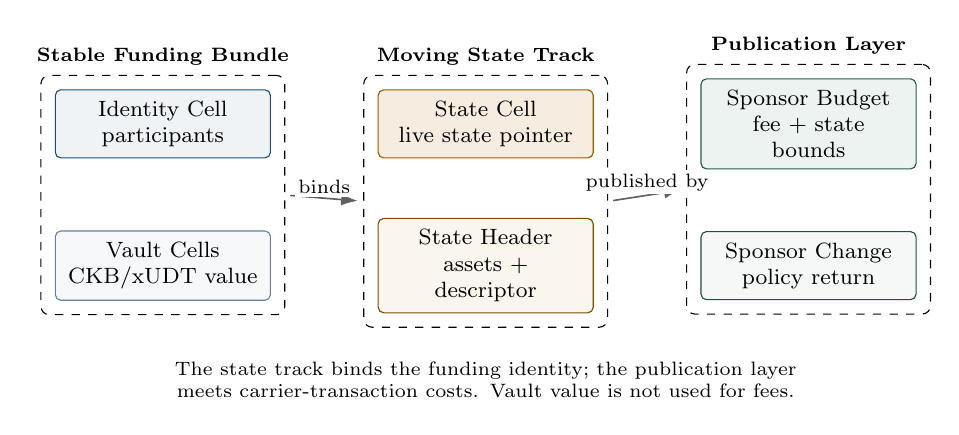
\begin{tikzpicture}[
  font=\footnotesize,
  box/.style={draw, rounded corners=2pt, align=center, text width=2.45cm, minimum height=0.72cm, inner sep=4pt},
  group/.style={draw, rounded corners=3pt, inner sep=5pt, dashed}
]
\node[box, fill=MorphBlue!7, draw=MorphBlue] at (0,0.9) (id) {Identity Cell\\participants};
\node[box, fill=MorphBlue!4, draw=MorphBlue!70] at (0,-0.9) (vaults) {Vault Cells\\CKB/xUDT value};
\node[group, fit=(id)(vaults), label={[font=\scriptsize\bfseries]above:Stable Funding Bundle}] (fundgroup) {};

\node[box, fill=MorphAmber!12, draw=MorphAmber!85!black] at (4.1,0.9) (scell) {State Cell\\live state pointer};
\node[box, fill=MorphAmber!7, draw=MorphAmber!70!black] at (4.1,-0.9) (commits) {State Header\\assets + descriptor};
\node[group, fit=(scell)(commits), label={[font=\scriptsize\bfseries]above:Moving State Track}] (stategroup) {};

\node[box, fill=MorphGreen!9, draw=MorphGreen!75!black] at (8.2,0.9) (budget) {Sponsor Budget\\fee + state bounds};
\node[box, fill=MorphGreen!5, draw=MorphGreen!65!black] at (8.2,-0.9) (change) {Sponsor Change\\policy return};
\node[group, fit=(budget)(change), label={[font=\scriptsize\bfseries]above:Publication Layer}] (sponsorgroup) {};

\draw[morpharrow] (fundgroup.east) -- node[arrowlabel, above]{binds} (stategroup.west);
\draw[morpharrow] (stategroup.east) -- node[arrowlabel, above]{published by} (sponsorgroup.west);
\node[align=center, font=\scriptsize, text width=8.7cm] at (4.1,-2.35)
  {The state track binds the funding identity; the publication layer meets carrier-transaction costs. Vault value is not used for fees.};
\end{tikzpicture}
\caption{Protocol object map. The funding bundle holds channel identity and value; the state track carries authority; the publication layer meets the transaction fee.}
\label{fig:object-map}
\end{figure}

\clearpage
\section{Script-Level Validation Semantics}

The following pseudo-code states the script checks required for an implementable construction. It is not byte-level CKB-VM code.

\begin{definition}[Canonical Operation Classification]
On-chain validation uses one canonical operation tag:
\[
\begin{aligned}
\mathsf{ChannelOperation}=\{&
\mathsf{FUND},\mathsf{PUBLISH},\mathsf{SUPERSEDE},
\mathsf{FINALIZE},\\
&\mathsf{COOPERATIVE\_CLOSE},\mathsf{SPLICE},
\mathsf{MATERIALIZE}\}.
\end{aligned}
\]
\[
\mathsf{OffchainEvent}=\{\mathsf{OFFCHAIN\_UPDATE}\}.
\]
Every on-chain transaction that touches a Morph State Cell, vault Cell,
descriptor output, or sponsor budget must carry or imply exactly one
\textsf{ChannelOperation}. The State Cell type script, vault lock, descriptor
parser, and sponsor policy must derive the same operation tag. If a transaction
admits two operation interpretations, it is invalid.
\end{definition}

\begin{definition}[Resolved State Context]
Header commitments are not the resolved protocol objects. A validator first
resolves the committed objects from the witness:
\begin{lstlisting}
resolve_state_context(header, witness):
  asset_registry =
    parse_and_verify_asset_registry(
      witness.asset_registry,
      header.asset_registry_commitment)
  descriptor =
    parse_and_verify_descriptor(
      witness.settlement_descriptor,
      header.settlement_descriptor_commitment,
      header.descriptor_version)
  challenge_policy =
    parse_and_verify_challenge_policy(
      witness.challenge_policy,
      header.challenge_policy_commitment)
  payload =
    parse_and_verify_payload_or_roots(
      witness.payload_or_roots,
      header.payload_commitment,
      header.mode)
  return ResolvedStateContext(
    header, asset_registry, descriptor,
    challenge_policy, payload)
\end{lstlisting}
All later validation rules use the resolved registry, descriptor, challenge
policy, and payload rather than treating commitments as full objects.
\end{definition}

\begin{figure}[H]
\centering
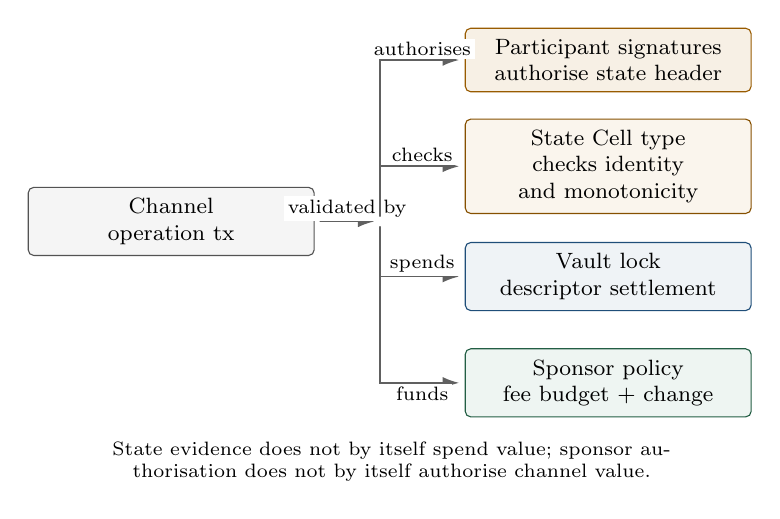
\begin{tikzpicture}[
  font=\footnotesize,
  box/.style={draw, rounded corners=2pt, align=center, text width=3.35cm, minimum height=0.72cm, inner sep=4pt}
]
\node[box, fill=gray!8, draw=gray!65!black] at (0,0) (tx) {Channel\\operation tx};
\node[box, fill=MorphAmber!10, draw=MorphAmber!85!black] at (5.55,2.05) (sig) {Participant signatures\\authorise state header};
\node[box, fill=MorphAmber!7, draw=MorphAmber!75!black] at (5.55,0.7) (state) {State Cell type\\checks identity and monotonicity};
\node[box, fill=MorphBlue!7, draw=MorphBlue] at (5.55,-0.7) (vault) {Vault lock\\descriptor settlement};
\node[box, fill=MorphGreen!8, draw=MorphGreen!75!black] at (5.55,-2.05) (sponsor) {Sponsor policy\\fee budget + change};

% Hub: tx feeds a validation bus that fans out to four independent checks
\coordinate (hub) at (2.65,0);
\draw[morpharrow] (tx.east) -- node[arrowlabel, above]{validated by} (hub);
\draw[morpharrow] (hub) |- node[arrowlabel, near end, above]{authorises} (sig.west);
\draw[morpharrow] (hub) |- node[arrowlabel, near end, above]{checks} (state.west);
\draw[morpharrow] (hub) |- node[arrowlabel, near end, above]{spends} (vault.west);
\draw[morpharrow] (hub) |- node[arrowlabel, near end, below]{funds} (sponsor.west);
\node[align=center, font=\scriptsize, text width=8.8cm] at (2.8,-3.05)
  {State evidence does not by itself spend value; sponsor authorisation does not by itself authorise channel value.};
\end{tikzpicture}
\caption{Authorisation boundaries for any value-touching channel operation. State signatures, vault spends, and sponsor fee authorisation are separate checks.}
\label{fig:authorisation-boundaries}
\end{figure}

\subsection{State Cell Type Semantics}

The State Cell type script is the sole script-level predicate for advancing or
retiring the live state track. It does not spend channel value; it verifies the
identity, monotonicity, and retirement conditions of state evidence. Ordinary
publication and supersession preserve the current funding epoch, funding
anchor, and vault-set commitment. Finalisation retires a settling State Cell
after the committed relative delay. A splice is a separate re-anchoring
transition: it must prove both the old and new funding context, rather than
silently changing these fields inside an ordinary state update.

\begin{table}[H]
\centering
\small
\setlength{\tabcolsep}{4pt}
\begin{tabular}{L{0.22\linewidth}L{0.22\linewidth}L{0.24\linewidth}L{0.22\linewidth}}
\toprule
Input phase & Output phase & Operation & Conservative rule \\
\midrule
none & active & \textsf{FUND} & create the genesis state-track pointer \\
active & settling & \textsf{PUBLISH} & publish pre-signed settlement evidence \\
settling & settling & \textsf{SUPERSEDE} & newer valid evidence replaces older evidence \\
settling & none & \textsf{FINALIZE} & mature state retires atomically over vault set \\
active or settling & none & \textsf{COOPERATIVE}\newline\textsf{CLOSE} & full close signatures; no challenge delay \\
active & active & \textsf{SPLICE} & signed re-anchor event updates funding context \\
factory-active & updated successor or retired & \textsf{MATERIALIZE} & resolved by the factory parent rule \\
settling & active & any & invalid \\
\bottomrule
\end{tabular}
\caption{State Header phase transition table. The \textsf{MATERIALIZE} row is resolved by the factory transition result.}
\label{tab:phase-transition}
\end{table}

\clearpage
\begin{lstlisting}
verify_state_cell_type(tx):
  op = classify_channel_operation(tx)

  if op == FUND:
    require zero_input_state_cells(tx, channel_id)
    new = exactly_one_output_state_cell(tx, channel_id)
    new_header = parse_state_header(new.data)
    resolved = resolve_state_context(new_header, witness)
    require new_header.channel_id == derived_channel_id(tx)
    require new_header.state_number == 0
    require new_header.phase == active
    require funding_anchor_derivation_matches(new_header, tx)
    require initial_configuration_signatures_valid(
            new_header, resolved.descriptor,
            resolved.asset_registry, resolved.challenge_policy,
            participants)
    require output_state_capacity_sufficient(new)

  if op in {PUBLISH, SUPERSEDE}:
    old = exactly_one_input_state_cell(tx, channel_id)
    new = exactly_one_output_state_cell(tx, channel_id)
    old_header = parse_state_header(old.data)
    new_header = parse_state_header(new.data)
    resolved = resolve_state_context(new_header, witness)

    require same_context_except_progress(old_header, new_header)
    require phase_transition_allowed(op, old_header.phase,
            new_header.phase)
    require descriptor_transition_admissible(
            old_header.settlement_descriptor_commitment,
            new_header.settlement_descriptor_commitment,
            old_header.descriptor_version,
            new_header.descriptor_version,
            witness)
    require new_header.state_number > old_header.state_number
    require new_header.phase == settling
    require referenced_funding_anchor(tx.cell_deps)
            matches new_header.funding_anchor_identity
    require signatures_valid(new_header, witness.signatures)
    require partition_conservation_for_publication(
            tx, resolved, op)
    require output_state_capacity_sufficient(new)

  if op == FINALIZE:
    state = exactly_one_input_state_cell(tx, channel_id)
    require zero_output_state_cells(tx, channel_id)
    input_header = parse_state_header(state.data)
    resolved = resolve_state_context(input_header, witness)
    require input_header.phase == settling
    require state_input_relative_block_since_satisfies(
            resolved.challenge_policy)
    require all_committed_vaults_consumed_or_evidenced(
            tx, input_header.vault_set_commitment,
            resolved.descriptor)
    require vault_finalisation_outputs_match_descriptor(
            tx, resolved.descriptor)
    require state_carrier_refund_matches_policy(tx)

  if op == COOPERATIVE_CLOSE:
    state = exactly_one_input_state_cell(tx, channel_id)
    require zero_output_state_cells(tx, channel_id)
            or exactly_one_terminal_receipt_cell(tx, channel_id)
    header = parse_state_header(state.data)
    resolved = resolve_state_context(header, witness)
    require header.phase in {active, settling}
    require cooperative_close_signatures_valid(tx, header)
    require cooperative_outputs_match_descriptor(
            tx, resolved.descriptor)
    require partition_conservation_for_close(
            tx, resolved, op)
    require state_carrier_refund_matches_policy(tx)

  if op == SPLICE:
    old = exactly_one_input_state_cell(tx, channel_id)
    new = exactly_one_output_state_cell(tx, channel_id)
    old_header = parse_state_header(old.data)
    new_header = parse_state_header(new.data)
    event = parse_signed_reanchor_event(tx.witness)
    require event.channel_id == old_header.channel_id
            == new_header.channel_id
    require event.old_funding_epoch == old_header.funding_epoch
    require event.new_funding_epoch
            == old_header.funding_epoch + 1
    require new_header.funding_epoch == event.new_funding_epoch
    require new_header.funding_anchor_identity
            == event.new_funding_anchor_identity
    require new_header.vault_set_commitment
            == event.new_vault_set_commitment
    require realised_new_vault_set_matches(tx.outputs, event)
    require consumed_old_vaults_match(tx.inputs, old_header)
    require splice_partition_conservation(tx, event.asset_deltas)
    require signatures_valid(event, required_participants)

  if op == MATERIALIZE:
    parent = exactly_one_input_state_cell(tx, channel_id)
    parent_header = parse_state_header(parent.data)
    factory = resolve_factory_context(parent_header, witness)
    require factory_materialisation_envelope_admissible(tx, factory)
    require local_proof_valid(tx, factory)
    require touched_rights_authorised(tx, factory)
    require non_interference_or_full_participant_signatures(
            tx, factory)
    require materialised_child_or_exit_outputs_match_descriptor(
            tx, factory)
    require factory.parent_state_rule
            in {updated_successor, retired}
    require parent_state_successor_rule_satisfied(tx, factory)
    require partition_conservation_for_materialisation(
            tx, factory, op)
\end{lstlisting}

The helper \texttt{same\_context\_except\_progress} is deliberately narrow:
protocol version, chain id, signature scheme, channel id, funding epoch,
funding anchor identity, vault-set commitment, participant commitment, asset
registry commitment, challenge-policy commitment, mode, and state-layout version
must remain equal. Only the state number, the phase transition admitted by
Table~\ref{tab:phase-transition}, the payload commitment, and an admissible
descriptor commitment/version transition may change.

The descriptor transition predicate is narrow. It permits a new
descriptor instance only when the new State Header is signed under the normal
state-signing domain and the descriptor version and grammar remain within the
protocol's accepted boundary. The vault later settles only against the
descriptor commitment in the authentic current live State Cell.

Splice validation is separate from ordinary monotonic publication. It must bind
the old funding anchor, the new funding anchor, the old vault-set commitment,
the new vault-set commitment, the base state number, the asset deltas, and the
participant signatures in one signed re-anchoring event. This prevents a
watchtower package or settlement descriptor from an earlier funding context
from being replayed after the channel has been resized.

The ``exactly one input, exactly one output'' rule is the script-level
expression of State Cell uniqueness for publication and supersession.
Finalisation is the explicit retirement branch: it consumes the settling State
Cell, checks maturity and vault materialisation, and creates no successor State
Cell. Mempool races are resolved by the ordinary CKB single-spend rule:
competing transactions may exist, but at most one can consume the current State
Cell on-chain.

\subsection{Vault Lock Semantics}

Vault locks own channel value. They must not accept a transaction merely because the transaction references the correct channel. They accept only settlement or materialisation authorised by the current state evidence.

\begin{lstlisting}
verify_vault_spend(tx):
  op = classify_channel_operation(tx)
  require op in {FINALIZE, COOPERATIVE_CLOSE, SPLICE, MATERIALIZE}

  state = exactly_one_authentic_input_state_cell(
            tx, channel_id, expected_state_type, expected_state_lock)
  header = parse_state_header(state.data)
  resolved = resolve_state_context(header, tx.witness)
  require header.funding_anchor_identity matches this_vault.channel
  require this_vault_membership_proof_matches(
            this_vault, tx.witness.vault_set,
            header.vault_set_commitment)

  if op == FINALIZE:
    require header.phase == settling
    require state_input_relative_block_since_satisfies(
            resolved.challenge_policy)
    require all_committed_vaults_consumed_or_evidenced(tx)

  if op == COOPERATIVE_CLOSE:
    require header.phase in {active, settling}
    require cooperative_close_signatures_valid(tx, header)
    require no_challenge_delay_required(tx)

  if op == SPLICE:
    require signed_reanchor_event(tx)
    require old_vault_consumed_according_to_old_vault_set(tx)
    require new_vault_outputs_match_signed_vault_set(tx)
    require signed_deltas_match_realised_cells(tx)

  if op == MATERIALIZE:
    require factory_materialisation_proof(tx)
    require parent_child_vault_descriptor_match(tx)
    require parent_state_successor_or_retirement_rule(tx)

  expected_outputs =
    derive_outputs(resolved.descriptor, resolved.payload, op)
  require canonical_outputs(tx.channel_outputs) == expected_outputs
  require partition_conservation(tx, resolved, op)
\end{lstlisting}

This lock is the point at which the current live state becomes economically meaningful. A State Cell without vault enforcement is only evidence; it does not protect value.

\subsection{Bounded Sponsor Budget Semantics}

A sponsor budget may be implemented as a standard wallet signature, a watchtower-owned Cell, or a bounded policy Cell. The bounded policy form is the most delicate because it authorises another actor to spend capacity for publication.

\begin{lstlisting}
verify_sponsor_budget_spend(tx):
  policy = parse_policy(this_budget_cell.data)
  op = classify_channel_operation(tx)
  header = parse_authoritative_operation_header(tx, op)

  require header.channel_id == policy.channel_id
  require relevant_state_cell_type_hash(tx, op)
          == policy.expected_state_type_hash
  require relevant_state_cell_lock_hash(tx, op)
          == policy.expected_state_lock_hash
  require policy.min_state_number <= header.state_number
  require header.state_number <= policy.max_state_number
  require tx_fee(tx) <= policy.max_fee_per_tx
  require policy.already_spent + tx_fee(tx)
          <= policy.max_total_fee
  require exactly_one_successor_budget_cell(tx)
  require successor.already_spent
          == policy.already_spent + tx_fee(tx)
  require sponsor_change_lock(tx) == policy.change_lock
  require no_channel_assets_in_sponsor_change(tx)
  require op in policy.allowed_operations
\end{lstlisting}

The authoritative operation header is the header that the State Cell branch
will validate. In the persisted-header profile, it is parsed from the relevant
input or output State Cell data according to the operation. In a
commitment-only profile, the witness header must hash to the State Cell's
persisted header commitment before the sponsor policy may inspect it. Sponsor
budget logic must not approve one witness header while the State Cell type
validates another.

A deployment may split sponsor budgets by fee-risk class. The conservative
profile distinguishes publication budgets for \textsf{PUBLISH}/\textsf{SUPERSEDE},
settlement budgets for \textsf{FINALIZE}/\textsf{MATERIALIZE}, and re-anchor
budgets for \textsf{SPLICE}. Each policy lists its allowed operations
explicitly.

The current devnet implementation uses the narrowest sponsor profile: sponsor
Cells pay only publication and supersession carrier fees for settling State Cell
outputs. They do not sponsor \textsf{FUND}, \textsf{FINALIZE},
\textsf{SPLICE}, \textsf{MATERIALIZE}, or \textsf{COOPERATIVE\_CLOSE}. The
broader operation-scoped budget forms above are deployment profiles that require
the sponsor script to resolve and check the authoritative operation context for
each admitted branch.

The cumulative \texttt{max\_total\_fee} predicate is script-enforceable only
for a stateful SponsorBudget Cell that is consumed exactly once and recreated
with the updated spent total. A normal wallet signature can enforce only the
current spend it signs. If no stateful budget Cell is present, total budget is
watchtower or wallet policy, not a consensus predicate.

Expiry windows, allowed sponsor sources, scan cadence, and webhook policy remain
operator or watchtower policy unless the deployment provides the script with verifiable
evidence for those fields. A bounded sponsor script rejects, or otherwise makes
inadmissible, a finite script-level deadline for which it cannot verify the
relevant chain evidence.

The policy is not an open wallet delegation. It is a bounded fee-spend right scoped to one channel, one state interval, and an explicit operation set.

\clearpage
\section{Protocol State Machine}

Let the channel phase be one of
\[
\mathsf{Phase} = \{\mathsf{funding},\mathsf{active},\mathsf{settling},\mathsf{closed}\}.
\]

\begin{figure}[H]
\centering
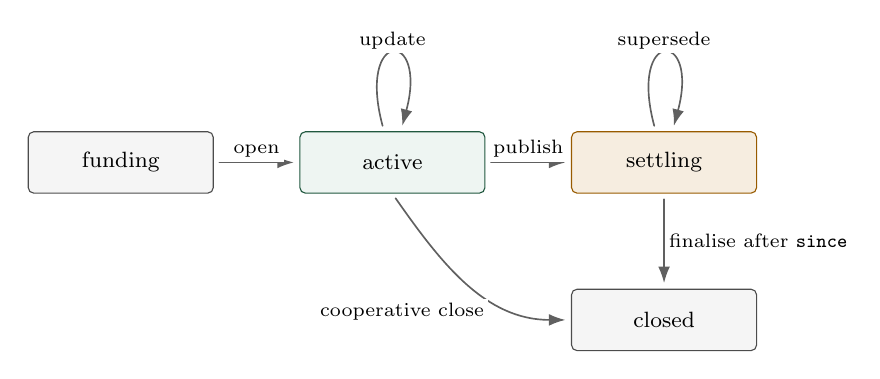
\begin{tikzpicture}[
  font=\footnotesize,
  box/.style={draw, rounded corners=2pt, align=center, minimum width=2.35cm, minimum height=0.78cm, inner sep=4pt},
  lab/.style={font=\scriptsize, fill=white, inner sep=1.5pt}
]
\node[box, fill=gray!8, draw=gray!60!black] at (0,0) (funding) {funding};
\node[box, fill=MorphGreen!8, draw=MorphGreen!70!black] at (3.45,0) (active) {active};
\node[box, fill=MorphAmber!12, draw=MorphAmber!85!black] at (6.9,0) (settling) {settling};
\node[box, fill=gray!8, draw=gray!60!black] at (6.9,-2.0) (closed) {closed};

\draw[morpharrow] (funding.east) -- node[lab, above, pos=0.50]{open} (active.west);
\draw[morpharrow] (active) to[loop above, min distance=1.35cm, looseness=8] node[lab]{update} (active);
\draw[morpharrow] (active.east) -- node[lab, above, pos=0.50]{publish} (settling.west);
\draw[morpharrow] (settling) to[loop above, min distance=1.35cm, looseness=8] node[lab]{supersede} (settling);
\draw[morpharrow] (settling.south) -- node[lab, right, align=center]{finalise after \texttt{since}} (closed.north);
\draw[morpharrow] (active.south) to[out=-55,in=180] node[lab, below left, pos=0.62]{cooperative close} (closed.west);
\end{tikzpicture}
\caption{Ordinary bilateral Morph Channel lifecycle. Publishing moves an active channel into the settling phase; newer signed evidence supersedes older settling evidence before finalisation. Splice and factory materialisation are separate paths.}
\label{fig:state-machine}
\end{figure}

The ordinary bilateral lifecycle contains the off-chain update event and five
on-chain branches:
\[
\begin{aligned}
&\mathsf{OFFCHAIN\_UPDATE};\\
&\mathsf{FUND},\quad
\mathsf{PUBLISH},\quad
\mathsf{SUPERSEDE},\quad
\mathsf{FINALIZE},\quad
\mathsf{COOPERATIVE\_CLOSE}.
\end{aligned}
\]
The full validation taxonomy additionally includes \textsf{SPLICE} and
\textsf{MATERIALIZE}. These are separate on-chain operation branches, not
ordinary bilateral state-machine arrows.

\clearpage
\section{Transaction Semantics}

\subsection{FUND}

\textsf{FUND} creates the stable funding bundle and the initial State Cell. The funding transaction may be funded by standard wallet inputs. After funding, channel-owned value enters the channel partition and should not be used for publication fees.

The initial State Cell is the only on-chain active pointer created by the channel. Its type arguments or equivalent identity mechanism must bind the same funding-anchor identity used by the Fund Cell and vault locks. A transaction that attempts to create two initial State Cells for the same channel genesis identity is invalid under the funding script profile.

\textsf{FUND} is outside unilateral dispute semantics. In the full protocol
profile it is authorised by the funding participants' normal wallet signatures
and by initial configuration signatures over the channel configuration,
\(\Header_0\), descriptor, asset registry, and challenge policy. The current
devnet implementation script-enforces anchor derivation, active phase, state
number zero, lock/type binding, and capacity shape; initial configuration
approval is host, wallet, and package policy rather than a separate
script-checked signature object. A stricter deployment may add explicit initial
configuration signature evidence without changing the State Header signing
domain. A sponsor may contribute fee-paying inputs, but that sponsorship does
not authorise the initial State Header or the vault configuration.

The initial active State Cell is not participant dispute evidence. It is the
genesis state-track pointer. Publishable off-chain updates use
\texttt{phase = settling}; the conversational fact that the participants still
consider the channel active is not part of the signed State Header.

\subsection{OFFCHAIN\_UPDATE}

An off-chain update produces a new publishable settlement-evidence object with a strictly larger state number. It does not consume CKB Cells. Participants exchange signatures over the canonical State Header whose \texttt{phase} is \texttt{settling} for unilateral publication. Any local ``active'' status recorded by a wallet or watchtower is conversational state outside the State Header signing domain. State numbers are strictly monotonic, but not necessarily consecutive: a valid supersession may move from $n$ to $n+k$ if the newer state is properly authorised and the sponsor policy admits that state interval.

Off-chain active updates do not create on-chain active State Cells. Once a unilateral publication reaches the chain, the channel is in the settling phase. Further on-chain progress is either supersession by a newer settling State Cell or finalisation after the relative challenge delay.

\subsection{PUBLISH and SUPERSEDE}

The same transaction pattern handles initial unilateral publication and challenge:
\begin{lstlisting}
PUBLISH_STATE:
  inputs:
    StateCell(n, active_or_settling)
    SponsorCell*
  cell_deps:
    FundingAnchor
    VaultCell*
  outputs:
    StateCell(n', settling)
    SponsorChange*
  validity:
    n' > n
    output StateCell(n', settling) persists
      or commits Header(n')
    signatures over canonical Header(n') are valid
    payload/proof resolves all Header commitments
    funding identity matches referenced anchor
    channel partition is conserved
\end{lstlisting}

Participant signatures authorise the state header. The transaction body selects live inputs, sponsor inputs, and fee rate, so a challenger may rebuild it against the currently live State Cell under competing tx-pool spends.

\begin{figure}[H]
\centering
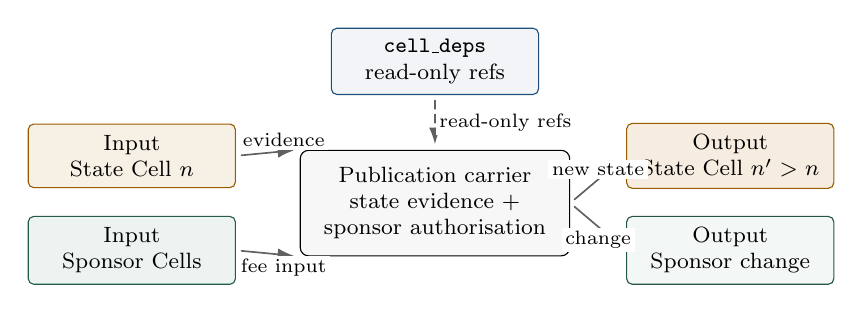
\begin{tikzpicture}[
  font=\footnotesize,
  box/.style={draw, rounded corners=2pt, align=center, text width=2.35cm, minimum height=0.72cm, inner sep=4pt},
  txbox/.style={draw, rounded corners=3pt, align=center, fill=gray!6, text width=3.0cm, minimum height=1.12cm, inner sep=6pt}
]
\node[box, fill=MorphAmber!10, draw=MorphAmber!85!black] at (0,0.45) (statein) {Input\\State Cell $n$};
\node[box, fill=MorphGreen!9, draw=MorphGreen!75!black] at (0,-0.75) (sponsorin) {Input\\Sponsor Cells};
\node[box, fill=MorphBlue!6, draw=MorphBlue] at (3.85,1.65) (deps) {\texttt{cell\_deps}\\read-only refs};

\node[txbox] at (3.85,-0.15) (tx) {Publication carrier\\state evidence + sponsor authorisation};

\node[box, fill=MorphAmber!12, draw=MorphAmber!85!black] at (7.6,0.45) (stateout) {Output\\State Cell $n' > n$};
\node[box, fill=MorphGreen!6, draw=MorphGreen!70!black] at (7.6,-0.75) (sponsorout) {Output\\Sponsor change};

\draw[morpharrow] (statein.east) -- node[arrowlabel, above, near end]{evidence} (tx.north west);
\draw[morpharrow] (sponsorin.east) -- node[arrowlabel, below, near end]{fee input} (tx.south west);
\draw[morphdash] (deps.south) -- node[arrowlabel, right, align=left]{read-only refs} (tx.north);
\draw[morpharrow] (tx.east) -- node[arrowlabel, above]{new state} (stateout.west);
\draw[morpharrow] (tx.east) -- node[arrowlabel, below]{change} (sponsorout.west);
\end{tikzpicture}
\caption{Publication and supersession transaction shape. The channel evidence can be reused while the sponsor inputs and fee choice are rebuilt.}
\label{fig:publish-transaction}
\end{figure}

\subsection{SPLICE}

\textsf{SPLICE} resizes a channel without closing its logical relationship. It is neither an ordinary off-chain update nor a final settlement. It is a signed re-anchoring transition that consumes the current active state and old vault authority, moves from the old funding context to a new funding context, and creates a new state and vault set for the same logical channel.

A splice-in increases the channel-controlled asset set by admitting external value. A splice-out releases value while preserving enough post-splice vault value to satisfy the latest signed settlement descriptor. In both cases, the signed transition must bind the old funding anchor, the new funding anchor, the old vault-set commitment, the new vault-set commitment, the base state number, and the per-asset deltas. The derived old and new funding context identifiers are useful package and watchtower keys, but they do not replace the underlying signed fields. CKB and xUDT lanes are checked by asset identity and amount, not by informal wallet labels.

The freshness consequence is material for recovery. A watchtower package saved before a splice is not automatically valid after the splice, even if it has a higher state number than some local record, because its signed funding context refers to a different enforceable value object. In the current implementation, ordinary state updates advance \texttt{state\_number} while keeping the funding context fixed; resize advances the funding context and signed funding epoch without requiring the channel's business state number to change.

\subsection{FINALIZE}

\textsf{FINALIZE} consumes the current settling State Cell and the committed vault set after the relative \texttt{since} delay has matured. It creates the settlement outputs authorised by the committed settlement descriptor. Retiring the state track without finalising or otherwise leaving verifiable finalisation evidence is invalid, because it would orphan channel value.

In the bilateral conservative profile, \textsf{FINALIZE} is atomic over the
entire committed vault set. Every live vault Cell committed by the current
State Header's \texttt{vault\_set\_commitment} must be consumed in the
finalisation transaction and materialised into descriptor-authorised outputs,
unless the descriptor explicitly proves that a vault is irrelevant and creates
a verifiable finalisation evidence object for any remaining value. Without
such a profile, partial finalisation is invalid.

If a profile admits non-atomic finalisation, its evidence object must be a
\texttt{TerminalReceipt}. The receipt binds the retired State Header, settlement
descriptor, finalised vault-set commitment, any remaining vault-set commitment,
and the carrier-refund output. The conservative bilateral profile does not rely
on this escape hatch: it consumes and materialises the entire committed vault
set atomically.
The current devnet implementation follows this conservative profile and does
not implement terminal receipts.

\subsection{COOPERATIVE\_CLOSE}

\textsf{COOPERATIVE\_CLOSE} is a terminal on-chain branch with explicit close
signatures from the required participants. It may consume an active or settling
State Cell, requires no challenge delay, and must still satisfy descriptor
materialisation, carrier-refund policy, and partition conservation. A
cooperative close is not a wallet-only spend of vault value; it is a
state-track retirement authorised by the channel participants.
The current devnet implementation models the operation in the host taxonomy but
does not implement a complete State type, vault contract, CLI, and devnet flow
for this branch. It is therefore a protocol branch and future deployment profile
rather than current executable evidence.

\subsection{MATERIALIZE}

\textsf{MATERIALIZE} is the factory-local branch that turns committed factory
rights into child-channel or local-exit Cells. It must resolve the factory
envelope, touched leaves, proof bundle, descriptor, asset registry, and
challenge policy before any value Cell is accepted. The parent factory State
Cell is consumed and either recreated with updated roots, retired, or paired
with a profile-defined terminal receipt. A proof that only changes a local
leaf is insufficient unless the rights-dependency schema proves that all
relevant untouched rights are unchanged.

For value-bearing \textsf{MATERIALIZE} in the conservative profile, the
resolved parent-state rule must be either \texttt{updated\_successor} or
\texttt{retired}. The \texttt{unchanged\_reference} rule is admissible only for
non-value-bearing proof queries or for a deployment profile whose vault lock
defines an alternative authority proof that does not require the parent State
Cell as an input.
The current factory implementation uses the \texttt{updated\_successor} path:
factory exits and reduced materialisation consume and recreate the parent
Factory State Cell with updated roots.

\clearpage
\section{Partition Conservation}

For every post-funding transaction, partition the transaction's values into channel-owned value $C$, State Cell carrier capacity $K$, and sponsor-owned value $S$. Read-only \texttt{cell\_deps} do not participate in value accounting. The high-level rule is operation-specific:
\[
\begin{aligned}
\textsf{PUBLISH/SUPERSEDE:}\quad &
C_{\mathrm{in}} = C_{\mathrm{out}},
\\[0.25em]
\textsf{FINALIZE:}\quad &
C_{\mathrm{in}} \mapsto
\mathrm{descriptor\_authorised\_settlement\_outputs},
\\[0.25em]
\textsf{SPLICE:}\quad &
C_{\mathrm{out}} =
C_{\mathrm{in}} + \Delta_{\mathrm{in}} - \Delta_{\mathrm{out}},
\\[0.25em]
\textsf{ALL:}\quad &
K_{\mathrm{in}} =
K_{\mathrm{state\_successor\_out}}+
K_{\mathrm{carrier\_refund\_out}},
\qquad
S_{\mathrm{in}} - S_{\mathrm{out}} = \mathrm{fee},
\\
&
C \cap K = K \cap S = C \cap S = \emptyset.
\end{aligned}
\]
In the conservative profile, State Cell carrier capacity is conserved exactly.
Finalisation may retire the State Cell only by creating a carrier-refund output
classified in the same $K$ lane. A deployment that wants sponsor-funded carrier
top-ups or carrier-cost deductions must add a separate signed carrier rule; it
must never charge the carrier delta to channel reserve or business CKB. Splice
deltas are signed protocol objects; every delta must bind asset type, amount,
capacity, Cell shape, and descriptor policy.

\begin{figure}[H]
\centering
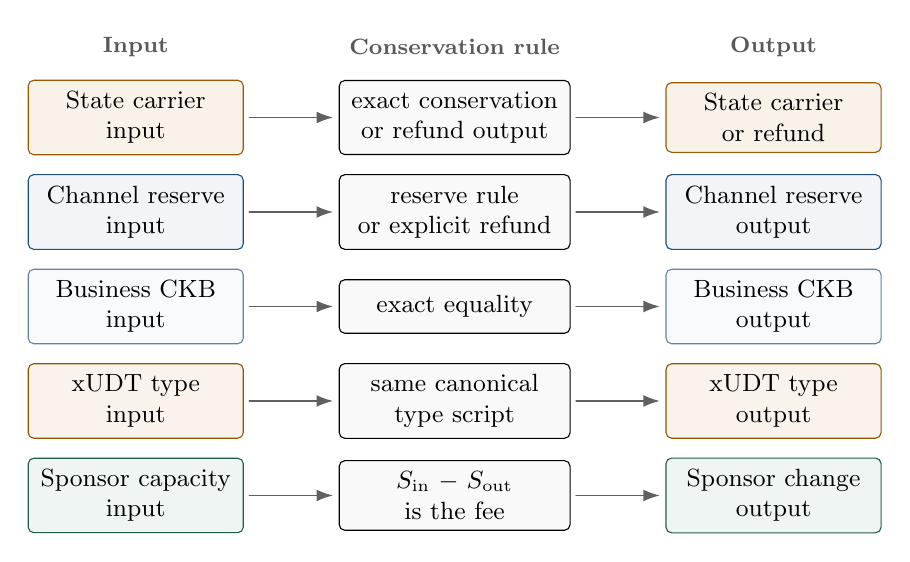
\begin{tikzpicture}[
  font=\small,
  lane/.style={draw, rounded corners=2pt, align=center, text width=2.45cm, minimum height=0.68cm, inner sep=4pt},
  rule/.style={draw, rounded corners=2pt, align=center, text width=2.65cm, minimum height=0.68cm, inner sep=4pt, fill=gray!5},
  colheader/.style={font=\footnotesize\bfseries, text=gray!70!black}
]
% Column headers
\node[colheader] at (0,4.05) {Input};
\node[colheader] at (4.05,4.05) {Conservation rule};
\node[colheader] at (8.1,4.05) {Output};

\node[lane, fill=MorphAmber!9, draw=MorphAmber!85!black] (kin) at (0,3.15) {State carrier\\input};
\node[rule] (krule) at (4.05,3.15) {exact conservation\\or refund output};
\node[lane, fill=MorphAmber!9, draw=MorphAmber!85!black] (kout) at (8.1,3.15) {State carrier\\or refund};

\node[lane, fill=MorphBlue!6, draw=MorphBlue] (rin) at (0,1.95) {Channel reserve\\input};
\node[rule] (rrule) at (4.05,1.95) {reserve rule\\or explicit refund};
\node[lane, fill=MorphBlue!6, draw=MorphBlue] (rout) at (8.1,1.95) {Channel reserve\\output};

\node[lane, fill=MorphBlue!3, draw=MorphBlue!70] (cin) at (0,0.75) {Business CKB\\input};
\node[rule] (crule) at (4.05,0.75) {exact equality};
\node[lane, fill=MorphBlue!3, draw=MorphBlue!70] (cout) at (8.1,0.75) {Business CKB\\output};

\node[lane, fill=MorphAmber!8, draw=MorphAmber!80!black] (uin) at (0,-0.45) {xUDT type\\input};
\node[rule] (urule) at (4.05,-0.45) {same canonical\\type script};
\node[lane, fill=MorphAmber!8, draw=MorphAmber!80!black] (uout) at (8.1,-0.45) {xUDT type\\output};

\node[lane, fill=MorphGreen!8, draw=MorphGreen!75!black] (sin) at (0,-1.65) {Sponsor capacity\\input};
\node[rule] (srule) at (4.05,-1.65) {$S_{\mathrm{in}}-S_{\mathrm{out}}$\\is the fee};
\node[lane, fill=MorphGreen!8, draw=MorphGreen!75!black] (sout) at (8.1,-1.65) {Sponsor change\\output};

\draw[morpharrow] (kin) -- (krule);
\draw[morpharrow] (krule) -- (kout);
\draw[morpharrow] (rin) -- (rrule);
\draw[morpharrow] (rrule) -- (rout);
\draw[morpharrow] (cin) -- (crule);
\draw[morpharrow] (crule) -- (cout);
\draw[morpharrow] (uin) -- (urule);
\draw[morpharrow] (urule) -- (uout);
\draw[morpharrow] (sin) -- (srule);
\draw[morpharrow] (srule) -- (sout);
\end{tikzpicture}
\caption{Partition conservation. State Cell carrier capacity, channel reserve, user-visible CKB, each xUDT type, and sponsor fees are checked as separate lanes.}
\label{fig:partition-conservation}
\end{figure}

\begin{invariant}[Partition Conservation]
Channel-owned value is exactly conserved across publication and challenge transactions, exactly materialised during finalisation, and changed during splice only by signed splice deltas. State Cell carrier capacity is accounted for in its own lane. Any publication-fee deficit is borne exclusively by the sponsor partition.
\end{invariant}

\subsection{Capacity-Aware Conservation Algorithm}

CKB capacity requires a finer rule than a single scalar balance. A channel-owned CKB Cell has two logically distinct components:
\[
\mathsf{capacity}(c)=
\mathsf{reserve}(c)+\mathsf{business\_ckb}(c),
\qquad
\mathsf{reserve}(c)\ge \mathsf{occupied}(c).
\]
The reserve component exists so the Cell can exist. The business component is user-visible CKB value. A valid transition must not silently convert reserve into fee, sponsor change, or business balance unless the descriptor explicitly authorises a reserve refund.

State Cell capacity is carrier capacity, not business value. The conservative
profile conserves this lane exactly: ordinary publication carries it into the
successor State Cell, and finalisation carries it into a carrier-refund output.
No State Cell carrier delta may be charged to \texttt{CHANNEL\_RESERVE} or
\texttt{BUSINESS\_CKB}.

For xUDT accounting, an asset type is the canonical identity of the full type script, for example the hash of its canonical encoding. It is not a symbol, name, display metadata, or wallet-level asset label.

\clearpage
\begin{lstlisting}
partition_conservation(tx, resolved, op):
  asset_registry = resolved.asset_registry
  descriptor = resolved.descriptor

  classify every input/output cell as:
    SPONSOR
    CHANNEL_RESERVE
    BUSINESS_CKB
    BUSINESS_XUDT(asset_type)
    STATE_CARRIER
    UNRELATED

  require UNRELATED cells are not loaded through script
          syscalls by State, vault, descriptor, sponsor,
          or xUDT checks
          and do not contribute to channel conservation
  require all channel output cells satisfy
          capacity(output) >= occupied_capacity(output)

  reserve_in  = sum(channel_reserve_amount(input))
  reserve_out = sum(channel_reserve_amount(output))
  authorised_reserve_refund =
    sum(outputs with role == RESERVE_REFUND
        and lock/type/capacity match
            descriptor.reserve_refund_policy)
  require reserve_out + authorised_reserve_refund == reserve_in

  carrier_in  = sum_capacity(state_carrier_inputs)
  carrier_out = sum_capacity(state_carrier_outputs)
  require carrier_out == carrier_in
  require carrier refund outputs are classified STATE_CARRIER
  require no carrier delta is charged to channel reserve
          or business CKB

  business_ckb_in  = sum(business_ckb_amount(input))
  business_ckb_out = sum(business_ckb_amount(output))
  require business_ckb_out == business_ckb_in

  for each asset_type in asset_registry.xudt_types:
    type_script = asset_registry.type_script(asset_type)
    require asset_type == hash(canonical(type_script))
    require sum_xudt(input, type_script)
            == sum_xudt(output, type_script)
    require every xUDT output for asset_type
            carries type_script

  require sponsor inputs are not classified as channel reserve
  sponsor_in  = sum_capacity(sponsor_inputs)
  sponsor_out = sum_capacity(sponsor_outputs)
  require sponsor_in - sponsor_out == tx_fee(tx)
  require sponsor_outputs carry no channel business assets
  require sponsor_outputs carry no registered xUDT type
  require sponsor_outputs do not use channel vault locks
  require sponsor_outputs have no descriptor output role
\end{lstlisting}

An output explicitly classified by the settlement descriptor is a channel or
settlement output, not sponsor change. Sponsor change is sponsor-owned capacity
only: it carries no channel vault lock, no registered xUDT type, no channel
business asset, and no descriptor output role.

The algorithm separates five questions that are otherwise readily conflated: whether the State Cell carrier has been preserved or refunded, whether channel reserve is conserved or refunded, whether CKB business value is conserved, whether each xUDT type is conserved under its own type script, and whether unrelated Cells are irrelevant. Unrelated Cells may appear only when they are irrelevant to channel script reads and irrelevant to conservation. They must not be loaded by State Cell type scripts, vault locks, descriptor parsers, sponsor policies, or xUDT composition checks as hidden witnesses for channel authority.

\begin{table}[t]
\centering
\small
\setlength{\tabcolsep}{4pt}
\begin{tabular}{p{0.18\linewidth}p{0.27\linewidth}p{0.34\linewidth}c}
\toprule
Partition & Source & Role & Fee payer \\
\midrule
Sponsor capacity & standard wallet or budget Cells & transaction fees and change & yes \\
State carrier capacity & State Cell and committed carrier refund & storage capacity for the moving state track & no \\
Channel reserve & channel-owned CKB capacity & Cell occupancy and reserve refund & no \\
Business assets & CKB or xUDT balances & participant settlement value & no \\
\bottomrule
\end{tabular}
\caption{Value partitions in Morph Channel.}
\label{tab:partitions}
\end{table}

\begin{proposition}[Zero Channel-Paid Publication Fees]
If partition conservation holds for a post-funding transaction, then publication fees cannot reduce channel-owned value.
\end{proposition}

\begin{proof}
CKB transaction fees are represented by the difference between input capacity and output capacity. Since State Cell carrier capacity, channel reserve, business CKB, and each registered xUDT type are conserved under their own lanes, no fee deficit can be charged to channel-owned value. The only permitted fee deficit is $S_{\mathrm{in}}-S_{\mathrm{out}}$, the sponsor partition.
\end{proof}

\clearpage
\section{Settlement Descriptor}

The settlement descriptor is a protocol object, not a general-purpose application language. It commits to the admissible output derivation rule for settlement and local materialisation. A minimal descriptor specifies:
\begin{enumerate}[label=(\arabic*)]
  \item participant destination policies;
  \item per-asset allocation rules;
  \item occupied-capacity requirements for outputs;
  \item reserve refund rules;
  \item required xUDT type scripts;
  \item sponsor change classification;
  \item descriptor version and upgrade boundary.
\end{enumerate}

\begin{definition}[Descriptor Grammar]
A descriptor instance is a canonical byte string under a versioned bounded
grammar:
\begin{lstlisting}
SettlementDescriptor {
  descriptor_version
  operation_scope
  output_count
  output[0..MAX_DESCRIPTOR_OUTPUTS]
  reserve_refund_policy
  carrier_refund_policy
  sponsor_change_policy
}

DescriptorOutput {
  role
  allowed_operations
  lock_hash
  capacity
  asset_kind
  type_script_hash_or_none
  amount
  data_commitment
}
\end{lstlisting}
The grammar admits only fixed families selected by \texttt{descriptor\_version}.
It contains no loops, no dynamic script dispatch, and no unbounded witness
program. The current bilateral profile uses fixed two-output CKB and CKB+xUDT
families; broader descriptor families require a new version and fresh
acceptance tests.

If \texttt{asset\_kind == XUDT}, \texttt{amount} is the canonical decoded
amount from output data under the registered xUDT data layout, and
\texttt{data\_commitment} commits either to the exact output data bytes or to
the canonical amount encoding selected by \texttt{descriptor\_version}. The
descriptor must state which rule applies.
\end{definition}

\begin{invariant}[Descriptor Boundedness]
The descriptor must authorise settlement, splice, factory materialisation, and reserve refund. It must not introduce unbounded application execution into channel witnesses.
\end{invariant}

\begin{invariant}[Exact Materialisation]
A signed descriptor or vault delta is not only an accounting statement. For every value-bearing Cell it authorises, the realised Cell must match the committed lock identity, capacity, type-script identity, and data-encoded amount. A proof that only one asset lane changed is insufficient if the resulting Cell shape can drift in an untouching lane.
\end{invariant}

\clearpage
\section{Bilateral Witness Mode}

For a two-party channel, the first witness format should remain plaintext. Bilateral state is typically small: balances, conditional payments, timeout information, and shutdown policies. Plaintext witnesses keep force-close transactions auditable and make early prototypes simpler to test. Privacy may later be improved by replacing the payload with committed state material once size and CKB-VM costs are measured.

Plaintext is not authority by itself. The authoritative object remains the signed state header and its payload commitment. A validator checks that the plaintext payload deterministically induces the committed payload hash and satisfies the descriptor and conservation rules.

The plaintext payload is a resolution object for \texttt{payload\_commitment},
not an alternative source of channel authority.

\clearpage
\section{Factory Proof Mode}

Factories require a different authority model. A factory may contain many participants, balances, subchannels, reserves, and local exit paths. Full plaintext disclosure on every local exit exposes unrelated participant data and may cause witness size and verification cost to grow with factory size. Factory authority should therefore be commitment-first.

\begin{definition}[Factory State]
A factory state is a state header plus a set of roots:
\begin{lstlisting}
FactoryState {
  state_header
  balances_root
  subchannels_root
  membership_root
  reserve_root
}
\end{lstlisting}
\end{definition}

\begin{definition}[Factory Transition Envelope]
A factory transition is admissible only after a bounded outer claim identifies its transition family and commits to exactly one evidence body:
\begin{lstlisting}
FactoryEnvelope {
  magic
  version
  kind
  flags
  body_len
  body_commitment
}
\end{lstlisting}
\end{definition}

The envelope is not the local proof. It is the admission-control object that specifies which proof grammar is being invoked and which evidence body is committed. The body commitment binds the full envelope interpretation context:
\[
\begin{aligned}
\mathsf{body\_commitment}
= \hash(&\texttt{"CKB\_MORPH\_FACTORY\_BODY\_V1"}\\
&\parallel \mathsf{magic}
\parallel \mathsf{version}
\parallel \mathsf{kind}
\parallel \mathsf{flags}\\
&\parallel \mathsf{body\_len}
\parallel \mathsf{body\_bytes}).
\end{aligned}
\]
The script checks \texttt{body\_len} before parsing the body. A body that merely parses as some factory payload is not authority unless the outer claim admits that transition family and binds that body.

\begin{definition}[Factory Body Bound]
\texttt{body\_len} is the on-chain byte-length bound. A deployment profile must
also specify the full body-bound profile used for acceptance testing:
\begin{lstlisting}
FactoryBodyBound {
  max_body_bytes
  max_touched_leaves
  max_proof_nodes
  max_cycles
  proof_family
}
\end{lstlisting}
The script must check \texttt{magic}, \texttt{version}, \texttt{kind},
\texttt{flags}, \texttt{max\_body\_bytes}, \texttt{body\_len}, and the body
commitment. The deployment may treat \texttt{max\_touched\_leaves},
\texttt{max\_proof\_nodes}, and \texttt{max\_cycles} as acceptance criteria
only if those bounds are not relied upon for authorisation safety. The proof
family must be script-visible or committed by the admitted envelope kind.
\end{definition}

\begin{definition}[Factory Transition Result]
A factory transition resolves to an explicit parent-state rule:
\begin{lstlisting}
FactoryTransitionResult {
  parent_state_rule:
    { unchanged_reference, updated_successor, retired }
  new_roots
  materialised_child_outputs
  remaining_factory_vault_outputs
}
\end{lstlisting}
For reduced local materialisation, the conservative profile uses
\texttt{updated\_successor}: the parent State Cell is consumed and recreated
with roots reflecting the removed or reduced local rights.
For value-bearing materialisation, \texttt{unchanged\_reference} is not a
conservative authority rule; it is reserved for read-only proof checks or for a
deployment profile with an explicit non-input vault-authority proof.
\end{definition}

\begin{definition}[Factory Witness]
A factory witness contains an outer transition envelope, an access manifest, a proof bundle, touched leaf payloads, and the required signatures:
\begin{lstlisting}
FactoryWitness {
  envelope
  state_header
  access_manifest
  proof_bundle
  touched_leaf_payloads
  signatures
}
\end{lstlisting}
\end{definition}

\begin{definition}[Transition Footprint]
The transition footprint of a factory action is the set of leaves read, written, inserted, removed, or proven absent by that action.
\end{definition}

\begin{definition}[Factory Right]
A factory right is any participant-relevant claim that may be changed by a local factory action:
\[
\mathsf{FactoryRight} =
\{\mathsf{balance},\mathsf{reserve\_claim},\mathsf{membership},
\mathsf{exit\_path},\mathsf{sponsor\_budget\_claim}\}.
\]
\end{definition}

\begin{definition}[Rights Dependency Schema]
A reduced factory transition is checked against a versioned rights-dependency
schema:
\begin{lstlisting}
RightsDependencySchema {
  schema_version
  roots
  dependency_edges: FactoryRightId -> DependencySet
}

DependencySet {
  direct_right
  shared_reserve
  membership
  exit_path
  sponsor_budget
  factory_vault_descriptor
}
\end{lstlisting}
For every untouched participant right, the proof must show that each dependency
named by the schema is unchanged or irrelevant to the admitted transition
family. If the proof cannot establish that fact, the transition is global and
requires full-participant authorisation.
\end{definition}

\begin{definition}[Non-Interference]
A factory action is non-interfering with respect to untouched participants if the proof bundle establishes that all their factory rights are unchanged, including rights that depend on shared reserve, membership, exit path, or public sponsor-budget state.
\end{definition}

A Merkle proof is insufficient unless the transition family also accounts for rights depending on reserve, membership, exit path, and sponsor-budget state. A touched balance leaf may also affect reserve liquidity, local exit eligibility, or sponsor-budget allocation. A proof of non-interference must either cover those dependencies or the action must fall back to full-participant authorisation. An envelope-first boundary prevents a reduced proof from being checked under a weaker authority rule.

\begin{figure}[H]
\centering
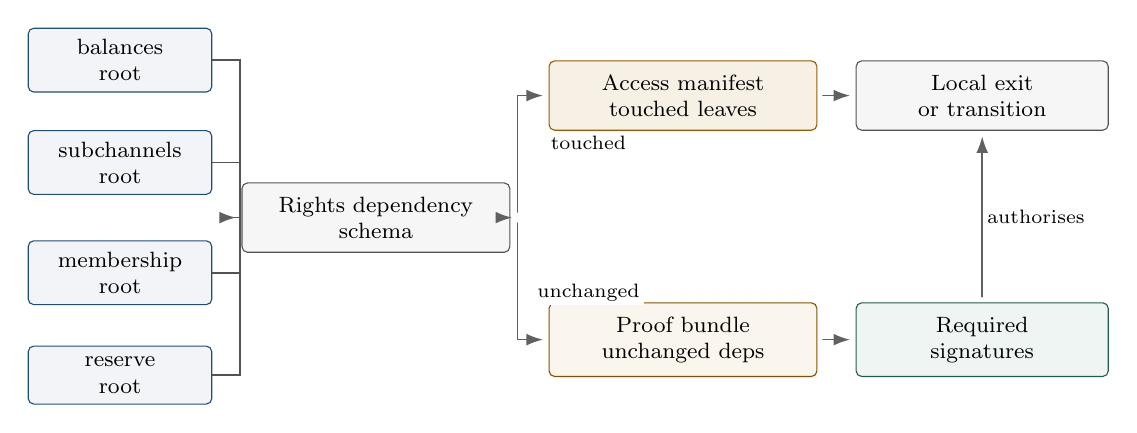
\begin{tikzpicture}[
  font=\footnotesize,
  box/.style={draw, rounded corners=2pt, align=center, text width=2.05cm, minimum height=0.60cm, inner sep=4pt},
  wide/.style={draw, rounded corners=2pt, align=center, text width=3.05cm, minimum height=0.82cm, inner sep=5pt},
  decision/.style={draw, rounded corners=2pt, align=center, text width=2.85cm, minimum height=0.86cm, inner sep=5pt},
  rootline/.style={-, semithick, draw=gray!65!black},
  chanlabel/.style={font=\scriptsize, fill=white, inner sep=1.5pt}
]
\node[box, fill=MorphBlue!6, draw=MorphBlue] at (0,2.0) (balances) {balances\\root};
\node[box, fill=MorphBlue!6, draw=MorphBlue] at (0,0.7) (subs) {subchannels\\root};
\node[box, fill=MorphBlue!6, draw=MorphBlue] at (0,-0.7) (members) {membership\\root};
\node[box, fill=MorphBlue!6, draw=MorphBlue] at (0,-2.0) (reserve) {reserve\\root};

\node[wide, fill=gray!7, draw=gray!65!black] at (3.25,0) (deps) {Rights dependency\\schema};
\node[wide, fill=MorphAmber!10, draw=MorphAmber!85!black] at (7.15,1.55) (manifest) {Access manifest\\touched leaves};
\node[wide, fill=MorphAmber!7, draw=MorphAmber!75!black] at (7.15,-1.55) (proof) {Proof bundle\\unchanged deps};
\node[decision, fill=gray!7, draw=gray!65!black] at (10.95,1.55) (exit) {Local exit\\or transition};
\node[decision, fill=MorphGreen!8, draw=MorphGreen!75!black] at (10.95,-1.55) (signers) {Required\\signatures};

% Merge bus: roots converge without arrowheads into a bus coordinate
\coordinate (rootbus) at (1.35,0);
\draw[rootline] (balances.east) -- ++(0.35,0) |- (rootbus);
\draw[rootline] (subs.east) -- ++(0.35,0) |- (rootbus);
\draw[rootline] (members.east) -- ++(0.35,0) |- (rootbus);
\draw[rootline] (reserve.east) -- ++(0.35,0) |- (rootbus);
\draw[morpharrow] (rootbus) -- (deps.west);

% Split bus: schema derives manifest (touched) and proof (unchanged)
\coordinate (split) at (5.05,0);
\draw[morpharrow] (deps.east) -- (split);
\draw[morpharrow] (split) |- (manifest.west);
\draw[morpharrow] (split) |- (proof.west);
\node[chanlabel] at (5.95,0.95) {touched};
\node[chanlabel] at (5.95,-0.95) {unchanged};

% Right side: manifest feeds exit, proof feeds signers, signers validate exit
\draw[morpharrow] (manifest.east) -- (exit.west);
\draw[morpharrow] (proof.east) -- (signers.west);
\draw[morpharrow] (signers.north) -- node[chanlabel, right, pos=0.50]{authorises} (exit.south);
\end{tikzpicture}
\caption{Factory proof mode. Roots feed the rights-dependency schema. The upper path exposes touched leaves for the local action; the lower path proves unchanged dependencies and admits the reduced signing set.}
\label{fig:factory-proof}
\end{figure}

\begin{proposition}[Conservative Factory Authorisation]
If a factory action cannot prove non-interference, then a conservative protocol profile should require signatures from all factory participants. If non-interference is proven, the signing set may be reduced to the affected participants only when the touched rights also satisfy participant authorisation, local validity, and value conservation.
\end{proposition}

\begin{proof}
Without non-interference, untouched leaves may still depend on shared membership, reserve, or exit-right state. A local signature set would not authorise those possible effects. Full-participant signatures authorise global effects. A non-interference proof removes only the effects on untouched rights; it does not by itself authorise minting a balance, increasing a reserve claim, deleting membership, or releasing value from a vault.
\end{proof}

\begin{proposition}[Envelope-First Factory Admissibility]
If the factory transition family is not fixed and committed before the local proof body is interpreted, then reduced authorisation is unsafe.
\end{proposition}

\begin{proof}
Different factory paths authorise different effects: a conservative update, a local exit, a single-right reduction, a sparse update, or a splice all have different admissible touched rights and value consequences. If the proof body determines its own authority class, an adversary may seek an alternative interpretation with weaker checks. A bounded outer claim fixes the transition family and commits to the body before local validity is evaluated, so the proof is checked under the intended authority rule only.
\end{proof}

\clearpage
\section{Factory Acceptance Requirements}

A deployment is not accepted merely because one representative factory path
succeeds. A candidate deployment must pass an end-to-end devnet acceptance
matrix in which every value-bearing factory flow is exercised as a
committed transition, and every attack-shaped factory rejection is checked
against its intended error class. The matrix is stated at protocol level
without prescribing a transaction builder, storage format, or proof encoding.

\begin{table}[htbp]
\centering
\small
\setlength{\tabcolsep}{4pt}
\begin{tabular}{L{0.30\linewidth}L{0.60\linewidth}}
\toprule
Factory flow family & Required positive acceptance evidence \\
\midrule
Factory lifecycle & factory creation; all-participant state advance; local child-channel materialisation; child publication; child finalisation \\
Reduced rights & bounded right decrease; tight near-zero decrease; sparse single-right update \\
CKB reduced exit & reserve-claim release into a local child channel; asymmetric participant capacity distribution \\
Typed reduced exit & partial xUDT release with factory-vault change; full xUDT release; one-sided xUDT settlement \\
Conservative factory splice & CKB splice-in and splice-out; asymmetric CKB capacity variants; xUDT splice-in and splice-out; one-sided xUDT variants \\
Reduced factory splice & CKB reduced splice-in and splice-out; asymmetric CKB variants; xUDT reduced splice-in and splice-out; one-sided xUDT variants \\
Sponsored factory publication & stateful budget publication; insufficient-budget rejection; valid later publication after sponsor failure \\
Recovery continuity & a valid later factory or child-channel transition remains publishable after an expected rejection \\
\bottomrule
\end{tabular}
\caption{Positive factory acceptance families. Every row is a required devnet acceptance family for a candidate deployment of the factory protocol.}
\label{tab:factory-acceptance-positive}
\end{table}

\begin{table}[htbp]
\centering
\small
\setlength{\tabcolsep}{4pt}
\begin{tabular}{L{0.30\linewidth}L{0.60\linewidth}}
\toprule
Factory rejection family & Required rejection evidence \\
\midrule
Factory lifecycle authority & stale, duplicate, or unauthorised state authority must not become value authority \\
Reduced locality & a locality proof must not authorise value creation or unrelated-right mutation \\
CKB reduced exit materialisation & released CKB and remaining reserve must match the authorised descriptor exactly \\
Typed reduced exit materialisation & mismatched typed settlement output or factory-vault typed change must be rejected \\
Conservative factory splice materialisation & vault descriptors and per-asset deltas must bind the realised Cell shape, not merely the aggregate amount \\
Reduced factory splice family confusion & sparse locality evidence must be checked under the admitted transition family only \\
Sponsor contamination & factory-local proof must not route channel xUDT or vault-locked capacity into sponsor change \\
Negative recovery continuity & attack-shaped typed materialisation failures must reject without poisoning later progress \\
\bottomrule
\end{tabular}
\caption{Factory rejection families. Every row is a required negative-path evidence family for a candidate deployment of the factory protocol.}
\label{tab:factory-acceptance-negative}
\end{table}

The acceptance rule is strict: every positive row in
Table~\ref{tab:factory-acceptance-positive} must be represented by committed
on-chain evidence, and every negative row in
Table~\ref{tab:factory-acceptance-negative} must be represented by an exact
rejection class. The non-interference proof must be accompanied by acceptance
evidence showing that conservative paths,
reduced paths, CKB paths, typed-asset paths, asymmetric value distributions, and
one-sided typed distributions all preserve the same authority and conservation
boundaries.

Committed on-chain evidence means a confirmed devnet transaction, or a rejected
devnet transaction attempt, whose transaction hash or rejection trace, script
error code, witness profile, envelope kind, and relevant State Header
commitment are recorded in the acceptance report.

\clearpage
\section{Challenge-Window Semantics}

The challenge window is a deployment parameter derived from CKB confirmation behaviour and watchtower liveness.

Let $\Delta$ denote the finalisation delay encoded by relative \texttt{since}. A conservative policy should satisfy:
\[
\Delta \ge
\Delta_{\mathrm{detect}}+
\Delta_{\mathrm{poll}}+
\Delta_{\mathrm{build}}+
\Delta_{\mathrm{confirm}}+
\Delta_{\mathrm{margin}}.
\]

The terms respectively represent detection confirmations, watchtower polling interval, transaction construction and propagation, confirmation of the newer-state transaction, and a margin for fee bumping and reorganisation risk. The current conservative profile uses a canonical relative block-number \texttt{since}. A future deployment may choose epoch- or timestamp-based maturity only if the mode, metric, reserved bits, and value are canonicalised and tested against current CKB hardfork semantics~\cite{ckb-since,ckb-since-timestamp,ckb-since-epoch}; raw integer comparison is not a valid challenge-window check.

\begin{table}[htbp]
\centering
\small
\setlength{\tabcolsep}{4pt}
\begin{tabular}{L{0.24\linewidth}L{0.32\linewidth}L{0.34\linewidth}}
\toprule
Parameter & Deployment evidence & Audit question \\
\midrule
Detection depth & chosen confirmation depth, for example 1, 3, or 6 confirmations & when does a watchtower treat stale evidence as actionable? \\
Polling interval & watchtower service objective & is there enough time between observation and finalisation? \\
Build and broadcast time & wallet, RPC, and network measurements & can a replacement carrier be assembled against the live State Cell? \\
Confirmation target & measured CKB confirmation behaviour & can the newer state confirm before the deadline? \\
Fee-bump margin & sponsor budget multiple & is there budget for conservative publication plus emergency rebuild? \\
Reorganisation margin & conservative deployment choice & does the delay tolerate expected reorg risk? \\
\bottomrule
\end{tabular}
\caption{Deployment profile required for selecting a challenge window.}
\label{tab:challenge-profile}
\end{table}

\begin{figure}[H]
\centering
\resizebox{0.96\linewidth}{!}{%
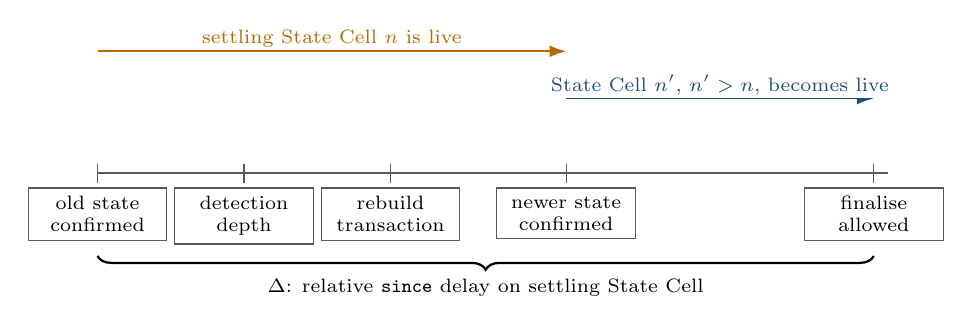
\begin{tikzpicture}[
  font=\footnotesize,
  x=0.93cm,
  y=1cm,
  timebox/.style={draw=gray!70!black, fill=white, align=center, text width=1.55cm, font=\scriptsize, minimum height=0.52cm, inner sep=3pt}
]
\draw[thick, gray!70!black] (0,0) -- (10.8,0);
\foreach \x/\lab in {
  0/{old state\\confirmed},
  2.0/{detection\\depth},
  4.0/{rebuild\\transaction},
  6.4/{newer state\\confirmed},
  10.6/{finalise\\allowed}
} {
  \draw[gray!70!black] (\x,0.12) -- (\x,-0.12);
  \node[timebox, below=0.18cm] at (\x,0) {\lab};
}
\draw[-{Latex[length=2.1mm,width=1.5mm]}, semithick, MorphAmber] (0,1.55) -- node[above, fill=white, inner sep=1pt, font=\scriptsize]{settling State Cell $n$ is live} (6.4,1.55);
\draw[-{Latex[length=2.1mm,width=1.5mm]}, semithick, MorphBlue] (6.4,0.95) -- node[above, fill=white, inner sep=1pt, font=\scriptsize]{State Cell $n'$, $n'>n$, becomes live} (10.6,0.95);
\draw[decorate, decoration={brace,mirror,amplitude=5pt}, thick]
  (0,-1.05) -- node[below=0.16cm, align=center, font=\scriptsize]{$\Delta$: relative \texttt{since} delay on settling State Cell} (10.6,-1.05);
\end{tikzpicture}%
}
\caption{Challenge-window timeline. Safety depends on confirmed supersession before the relative finalisation delay matures, not on tx-pool visibility alone.}
\label{fig:challenge-window}
\end{figure}

\subsection{CKB \texttt{since} and Mempool Reality}

In CKB, relative \texttt{since} is checked on transaction inputs. For Morph finalisation, the relevant input is the currently live settling State Cell. Therefore a finalisation transaction should set \texttt{since} on the State Cell input and the State type or vault lock should check that the value is an encoded relative-block condition matching the committed challenge policy. A naked numeric value is not equivalent to a relative delay. The finalisation deadline is computed from the confirmed block or epoch position of the live settling State Cell input according to the committed since metric, not from a watchtower's observation time.

The safety condition is confirmation before the deadline, not mempool presence. A challenger may observe an old state in the tx-pool, but the protocol need not respond until an old settling State Cell is actually confirmed or reaches the configured detection depth. If the old state confirms, the challenger rebuilds a newer-state transaction against the now-live settling State Cell. If a newer-state transaction remains unconfirmed, the watchtower must be able to rebuild it with different sponsor inputs or a higher fee, because the channel signature does not commit to sponsor coin selection.

Fee bumping does not rely on Bitcoin-style replace-by-fee semantics. It means reconstructing a fresh transaction body against the current live State Cell and current sponsor funds. Once a competing transaction consumes that State Cell, all stale transaction bodies become invalid and must be rebuilt.

\begin{lstlisting}
watchtower_response_loop:
  observe chain tip and tx-pool
  if confirmed settling StateCell(n) reaches detection_depth:
    latest = local_state_package(channel_id)
    if latest.state_number > n:
      tx = build_publish_state_tx(
             input_state = live StateCell(n),
             state_package = latest,
             sponsor_policy = available_budget(),
             fee_rate = conservative_fee_rate())
      broadcast(tx)
      while tx not confirmed
            and blocks_until_deadline(live StateCell(n))
                > emergency_rebuild_margin:
        if fee market or sponsor set changes:
          tx = rebuild_against_live_state_cell()
          broadcast(tx)
\end{lstlisting}

The watchtower policy must reserve enough fee budget for at least one conservative publication and one emergency rebuild. If the deployment expects volatile fees, the budget should support additional rebuild attempts. This is an operational requirement.

\begin{proposition}[Newer-State Supersession]
Suppose a settling State Cell at number $n$ is live. If an honest party publishes and confirms valid evidence $E_{n'}$ with $n'>n$ before finalisation of $E_n$, then $E_n$ cannot be the final settlement authority.
\end{proposition}

\begin{proof}
The supersession transaction consumes the live settling State Cell at $n$ and creates a new settling State Cell at $n'$. Once consumed, the $n$ State Cell cannot be used as an input to finalisation. The finalisation rule applies only to the currently live settling State Cell after its own relative \texttt{since} delay matures.
\end{proof}

\clearpage
\section{Signature Domains and Authorisation Boundaries}

Morph separates three authorisation domains:
\begin{enumerate}[label=(\arabic*)]
  \item state authorisation: participant signatures over the canonical State Header;
  \item value authorisation: vault locks accepting only descriptor-authorised settlement or materialisation;
  \item fee authorisation: sponsor signatures or bounded sponsor policies.
\end{enumerate}

\begin{lemma}[Domain-Separated Anti-Replay]
If protocol version, signature-scheme identity, chain identity, channel identity, funding epoch, funding anchor identity, vault-set commitment, mode, phase, participants commitment, asset registry, descriptor commitment, descriptor version, challenge policy, and state number are included in the signed State Header, then a valid state signature cannot be replayed as a valid state for another channel context, funding context, or later protocol interpretation.
\end{lemma}

\begin{proof}
Any change to the protocol version, signature scheme, chain, channel, funding epoch, funding anchor, vault set, mode, phase, participants, asset registry, descriptor, descriptor version, challenge policy, or state number changes the canonical State Header and hence the signed message. Under signature unforgeability, the adversary cannot produce a valid participant signature for the modified context.
\end{proof}

\clearpage
\section{Watchtower and Recovery Objects}

A watchtower stores the latest state package and publishes newer evidence when stale evidence appears on-chain; it never receives authority over channel-owned value. A state package contains more operational material than a bare root, but less disclosure than a permanent plaintext dump:
\begin{lstlisting}
StatePackage {
  header
  payload_or_roots
  proof_package
  participant_signatures
  resolved_descriptor_or_descriptor_bytes
  resolved_asset_registry
  resolved_challenge_policy
  sponsor_policy_reference
}
\end{lstlisting}
The package must resolve every commitment required by the selected State Header
representation profile. A header and signatures alone are insufficient if the
publication path also needs descriptor bytes, asset registry bytes, challenge
policy bytes, or factory proof material.
The current bilateral devnet package is narrower than this abstract object: it
stores the signed header bytes, bilateral signature witness bytes, channel id,
funding anchor, derived funding context id, state number, signing digest,
source State outpoint, and descriptor commitment/version metadata. It validates
the signatures and metadata for the plaintext bilateral profile. Broader
packages that carry explicit generic asset-registry bytes, challenge-policy
bytes, or commitment-only proof material remain representation-profile work.

The script-enforced sponsor boundary must be bounded by channel identity, state-number range, maximum fee, expected State Type, and change destination. Expiry windows, allowed sponsor sources, and publishing cadence are operator or watchtower policy in the conservative profile unless a deployment provides script-verifiable evidence for those fields; finite script-level deadlines without such evidence should be rejected rather than treated as consensus-enforced policy. The watchtower must not be able to redirect channel-owned value or drain arbitrary wallet funds.

After a splice, watchtower recovery must be funding-context aware. A stored package is publishable only if its signed funding context matches the currently live state track. Tooling should prefer the derived \texttt{funding\_context\_id} for package selection and cursor recovery, while retaining a funding-anchor fallback only for older package stores that predate the derived identifier. A package whose funding context does not match the live State Cell is merely historical evidence for an older funding context.

\clearpage
\section{Safety Properties}

\begin{proposition}[Funding Context Uniqueness]
If the State Header binds the funding epoch, funding anchor identity, and vault-set commitment, and scripts verify that referenced \texttt{cell\_deps} match that context, then a descriptor-shaped but non-authoritative Cell cannot serve as the channel's funding anchor or vault set.
\end{proposition}

\begin{proof}
The script compares the referenced Cell identity and vault-set commitment with the context committed in the State Header. A different Cell, even with similar data, has a different outpoint, genesis identity, or vault-set commitment and is rejected.
\end{proof}

\begin{proposition}[Post-Splice Freshness]
If a splice advances the funding epoch and commits to a new vault set, then a state package from an earlier funding epoch cannot authorise settlement of the post-splice vaults.
\end{proposition}

\begin{proof}
The earlier package signs a different funding epoch, funding anchor, or vault-set commitment. Since vault settlement requires the authentic current live State Cell and the descriptor bound to that funding context, the older package does not match the post-splice value object.
\end{proof}

\begin{proposition}[Vault Spend Safety]
If each vault lock accepts only settlement transactions, and materialisation transactions for deployment profiles that define the \textsf{MATERIALIZE} State Cell branch, authorised by an authentic current live State Cell and descriptor-admissible outputs, then channel-owned value cannot be spent through standard wallet paths or fake state-header bytes.
\end{proposition}

\begin{proof}
Every spend of channel-owned value must satisfy the vault lock. By assumption, the lock rejects transactions lacking authentic current state evidence and descriptor-admissible outputs. Ordinary wallet signatures alone are insufficient, and a non-authoritative Cell that only imitates the State Header layout does not satisfy the state-evidence predicate.
\end{proof}

\begin{proposition}[Recoverable Unilateral Settlement]
If a participant or watchtower stores a valid State Package that resolves every commitment required by the selected representation profile, has access to sponsor funds within policy, and the challenge delay satisfies the response-budget inequality, then it can reconstruct a publication transaction without fresh counterparty cooperation.
\end{proposition}

\begin{proof}
The channel signature excludes sponsor inputs and fee rate, so the publication transaction may be rebuilt using available sponsor funds. The State Package supplies the signed state evidence and required witness or proof. The response-budget inequality provides time for detection, construction, propagation, and confirmation.
\end{proof}

\clearpage
\section{Evaluation Agenda}

Empirical closure requires the following benchmark evidence:
\begin{enumerate}[label=E\arabic*.]
  \item bilateral plaintext witness size under realistic payment states;
  \item factory proof size under realistic touched-footprint distributions;
  \item CKB-VM cycles for signature verification, hash verification, proof verification, and xUDT type-script composition;
  \item challenge reliability under confirmation-depth, fee-volatility, and watchtower-polling parameters;
  \item sponsor-policy failure cases, including insufficient budget, inadmissible finite script-level expiry, operator-level expiry, and wrong change destination;
  \item State Cell uniqueness tests under concurrent publication and supersession attempts;
  \item splice freshness tests showing that packages from earlier funding epochs cannot govern later vault sets;
  \item vault-lock rejection tests for spends lacking current state evidence;
  \item descriptor grammar tests for output-count bounds, version boundaries, carrier-refund policy, and forbidden dynamic dispatch;
  \item State Cell carrier-capacity, reserve refund, occupied-capacity, business-CKB, and per-xUDT conservation edge cases;
  \item factory envelope-admission tests for transition-family confusion, body-bound violations, and digest mismatch;
  \item factory acceptance and rejection evidence for every lifecycle, reduced-rights, reduced-exit, conservative-splice, reduced-splice, asymmetric, and one-sided typed path in Tables~\ref{tab:factory-acceptance-positive} and~\ref{tab:factory-acceptance-negative};
  \item executable negative tests corresponding to the audit matrix in Appendix~\ref{app:audit-matrix};
  \item comparison between full plaintext factory disclosure and local proof verification.
\end{enumerate}

\clearpage
\section{Related Work and Positioning}

Lightning~\cite{lightning} represents the penalty-based payment-channel family. Eltoo~\cite{eltoo} provides the update-by-replacement intuition, but depends on Bitcoin sighash changes. Channel factories~\cite{factories} motivate shared funding and local exit questions. State-channel frameworks such as Perun~\cite{perun} show the broader adjudication pattern in which off-chain evidence is made enforceable by an on-chain dispute procedure. CKB community work on generic payment channels~\cite{ckb-gpc} is a nearer point of comparison, because it studies channel composability directly on the Cell model.

CKB's Cell model~\cite{ckb-cell} and transaction structure~\cite{ckb-tx} provide explicit state objects and read-only dependency references. CKB's \texttt{since} field~\cite{ckb-since,ckb-since-timestamp,ckb-since-epoch} provides relative lock semantics needed for challenge windows. SUDT~\cite{sudt} and xUDT~\cite{xudt} motivate per-asset conservation rather than a single undifferentiated balance.

\begin{table}[htbp]
\centering
\small
\setlength{\tabcolsep}{3pt}
\begin{tabular}{L{0.15\linewidth}L{0.22\linewidth}L{0.20\linewidth}L{0.15\linewidth}L{0.18\linewidth}}
\toprule
Work & Funding and state shape & Dispute rule & Fee model & Morph distinction \\
\midrule
Lightning & funding output plus commitment transactions & stale states are penalised & fees are carried by commitment or closing transactions & separates State Cell evidence from vault value \\
eltoo & replacement-style update state over a funding output & newer state replaces older state & depends on transaction form and proposed sighash support & borrows the replacement intuition, not the Bitcoin mechanism \\
Channel factories & shared funding for many off-chain relationships & local exits depend on factory validity rules & not the central object & adds envelope-first local proof admission and non-interference tests \\
Perun & adjudicated state-channel framework & on-chain dispute procedure enforces off-chain evidence & framework-dependent & specialises the adjudication object to CKB Cells and vault locks \\
CKB generic channels & Cell-based channel composability & CKB script enforcement & CKB transaction fees & adds sponsor partitioning, splice freshness, and per-asset conservation \\
\bottomrule
\end{tabular}
\caption{Positioning against related channel constructions.}
\label{tab:related-work}
\end{table}

Morph occupies a narrower point in this design space: CKB can host a channel object whose funding identity, state evidence, fee publication, and factory-local proof objects are separated at the script level without changing base-layer consensus.

\clearpage
\section{Limitations and Open Questions}

The construction remains incomplete in several respects:
\begin{enumerate}[label=O\arabic*.]
  \item Factory coordination remains an off-chain protocol problem.
  \item Proof mode may not be cheaper than plaintext until measured.
  \item Mainnet challenge delays require empirical confirmation and fee data.
  \item Descriptor versioning must balance upgrade flexibility against recoverability.
  \item Different xUDT variants may impose different constraints.
  \item The paper now specifies protocol-level validation semantics, but not every deployment-level encoding or operational procedure.
  \item Factory non-interference still requires mechanised coverage of the rights-dependency schema before reduced signing sets are safe in broader transition families.
  \item Factory envelope families and proof-size bounds require continued measurement under realistic transition mixes.
  \item Typed reduced exits and typed factory vault changes are admissible only when asset type, amount, capacity, child or factory vault Cell shape, settlement descriptor, and factory-vault change are completely bound. Broader typed-asset compatibility remains future work.
  \item Cooperative close, non-publication sponsor budgets, and any stricter script-checked \textsf{FUND} configuration signature profile require deployment-specific branch encodings before the construction is implementation-complete.
  \item Commitment-only profiles require deployment-specific resolution rules for asset registries, descriptors, payloads, and challenge policies.
\end{enumerate}

\clearpage
\section{Conclusion}

Morph Channel sets out how to separate funding identity, state evidence, sponsor
fee responsibility, and factory-local proof admission using current CKB script
objects. The construction keeps channel value in vault Cells, moves dispute
authority through a State Cell, checks channel and sponsor value in separate
partitions, and requires factory-local proofs to be admitted by a bounded
transition envelope.

The remaining burden is empirical and operational. A deployable protocol requires
benchmark evidence for witness size, CKB-VM cycles, challenge-window
parameters, fee-budget policy, splice recovery, and factory proof costs. Until
those measurements exist, Morph remains a script-level construction for CKB
channels rather than a production channel network.

\appendix

\clearpage
\section{Audit Matrix}
\label{app:audit-matrix}

This appendix states the construction audit target in testable form. The matrix
is split by authority boundary so that each row remains reader-facing rather
than an internal QA spreadsheet. Each row should become at least one positive
test and one negative test in any candidate deployment.

\begin{table}[H]
\centering
\footnotesize
\setlength{\tabcolsep}{4pt}
\begin{tabular}{L{0.06\linewidth}L{0.34\linewidth}L{0.27\linewidth}L{0.25\linewidth}}
\toprule
ID & Invariant and enforcement & Positive case & Negative case \\
\midrule
S1 & One live State Cell controls the channel pointer; enforced by the State Cell type and CKB single-spend & supersede $n \rightarrow n+1$ by consuming the current State Cell & transaction creates two successor State Cells \\
S2 & Funding anchor identity is canonical; enforced by the State Header and \texttt{cell\_deps} check & referenced anchor matches committed genesis identity & descriptor-shaped fake anchor is referenced \\
S3 & State numbers are strictly monotonic; enforced by the State Cell type script & supersede $n \rightarrow n+k$ with valid signatures & publish lower or equal state number \\
S4 & State retirement does not orphan value; enforced by State and vault authority coupling & retirement finalises value or leaves verifiable finalisation evidence & State Cell is consumed while matching vault value remains live without evidence \\
S5 & Splice advances funding context without changing channel identity; enforced by signed old/new funding anchors, vault-set commitments, and funding epoch generation label & post-splice state binds new anchor and vault set & pre-splice package controls post-splice vaults \\
\bottomrule
\end{tabular}
\caption{State and funding audit matrix.}
\label{tab:audit-state-funding}
\end{table}

\begin{table}[H]
\centering
\footnotesize
\setlength{\tabcolsep}{4pt}
\begin{tabular}{L{0.06\linewidth}L{0.34\linewidth}L{0.27\linewidth}L{0.25\linewidth}}
\toprule
ID & Invariant and enforcement & Positive case & Negative case \\
\midrule
V1 & Vault value follows current state evidence; enforced by the vault lock and settlement descriptor & finalise after valid \texttt{since} delay & wallet-only spend of vault value \\
V2 & Vault authority requires an authentic State Cell; enforced by State/Vault script identity checks & State Cell under expected scripts controls finalise & ordinary Cell carries decodable State Header bytes \\
V3 & Descriptor evolution is signed state semantics; enforced by State signature and descriptor commitment & newer signed state commits to an admissible descriptor instance & finalise supplies an unsigned replacement descriptor \\
D1 & Descriptor grammar is bounded and versioned; enforced by descriptor parser and version gate & fixed two-output CKB or CKB+xUDT descriptor parses under its version & descriptor body invokes dynamic dispatch or exceeds output bound \\
\bottomrule
\end{tabular}
\caption{Vault and descriptor audit matrix.}
\label{tab:audit-vault-descriptor}
\end{table}

\begin{table}[H]
\centering
\footnotesize
\setlength{\tabcolsep}{4pt}
\begin{tabular}{L{0.06\linewidth}L{0.34\linewidth}L{0.27\linewidth}L{0.25\linewidth}}
\toprule
ID & Invariant and enforcement & Positive case & Negative case \\
\midrule
P1 & Channel-owned capacity never pays publication fees; enforced by partition conservation & sponsor capacity pays fee and receives change & reserve reduced by transaction fee \\
K1 & State carrier capacity is conserved independently; enforced by the State carrier lane & State Cell capacity moves to successor or carrier-refund output & State Cell capacity is silently consumed as a fee \\
P2 & Reserve and business CKB are not confused; enforced by reserve and business-CKB ledgers & authorised reserve refund is explicit & reserve becomes hidden business balance or fee \\
X1 & xUDT value is conserved by canonical type script; enforced by asset registry and xUDT type check & same canonical type script and amount & same symbol or metadata with different type script \\
G1 & Sponsor change is uncontaminated; enforced by sponsor policy and partition classifier & sponsor change contains only sponsor capacity & sponsor change carries registered xUDT or vault lock \\
G2 & Unverifiable sponsor deadlines are not script policy; enforced by the sponsor-policy boundary & unbounded script policy or verifiable deadline evidence & finite deadline is accepted without chain-verifiable evidence \\
U1 & Unrelated Cells cannot influence channel validity; enforced by script read set and conservation classifier & unrelated wallet input pays no channel role & helper Cell is read by channel scripts without classification \\
\bottomrule
\end{tabular}
\caption{Fee, capacity, and asset audit matrix.}
\label{tab:audit-fee-assets}
\end{table}

\begin{table}[H]
\centering
\footnotesize
\setlength{\tabcolsep}{4pt}
\begin{tabular}{L{0.06\linewidth}L{0.34\linewidth}L{0.27\linewidth}L{0.25\linewidth}}
\toprule
ID & Invariant and enforcement & Positive case & Negative case \\
\midrule
C1 & Challenge safety is confirmation-based; enforced by deployment profile and \texttt{since} policy & newer state confirms before deadline & stale state finalises while newer transaction is only in mempool \\
C2 & Challenge maturity is canonical relative block \texttt{since}; enforced by State/Vault since parser & encoded relative block delay matures & raw absolute integer is accepted as a delay \\
\bottomrule
\end{tabular}
\caption{Challenge-window audit matrix.}
\label{tab:audit-challenge}
\end{table}

\begin{table}[H]
\centering
\footnotesize
\setlength{\tabcolsep}{4pt}
\begin{tabular}{L{0.06\linewidth}L{0.34\linewidth}L{0.27\linewidth}L{0.25\linewidth}}
\toprule
ID & Invariant and enforcement & Positive case & Negative case \\
\midrule
F1 & Factory locality preserves untouched rights; enforced by proof bundle and rights-dependency graph & touched leaves prove affected rights only & shared reserve or exit right changes without authorisation \\
F2 & Factory locality is not mint authority; enforced by local validity and conservation predicates & value right decreases or vault-delta-bound increases & Merkle-only proof increases ReserveClaim or Balance \\
F3 & Factory vault materialisation matches signed descriptors; enforced by descriptor and delta materialisation checks & FactoryVault capacity, type, and amount match the signed descriptor & xUDT token delta is correct but recreated FactoryVault capacity drifts \\
F4 & Factory transition family is fixed before proof interpretation; enforced by bounded outer claim plus body commitment & admitted local proof is checked under its declared family & same proof body is reinterpreted as a weaker path \\
\bottomrule
\end{tabular}
\caption{Factory audit matrix.}
\label{tab:audit-factory}
\end{table}

\clearpage
\begin{thebibliography}{10}
\raggedright

\bibitem{lightning}
Joseph Poon and Thaddeus Dryja.
\newblock The Bitcoin Lightning Network: Scalable Off-Chain Instant Payments.
\newblock \url{https://lightning.network/lightning-network-paper.pdf}.

\bibitem{eltoo}
Christian Decker, Rusty Russell, and Olaoluwa Osuntokun.
\newblock eltoo: A Simple Layer2 Protocol for Bitcoin.
\newblock \url{https://blockstream.com/eltoo.pdf}.

\bibitem{factories}
Conrad Burchert, Christian Decker, and Roger Wattenhofer.
\newblock Scalable Funding of Bitcoin Micropayment Channel Networks.
\newblock \url{https://tik-old.ee.ethz.ch/file//49218d6b9325ddb4f18aef8830ec567b/1/scalable_funding.pdf}.

\bibitem{perun}
Stefan Dziembowski, Lisa Eckey, Sebastian Faust, and Daniel Malinowski.
\newblock Perun: Virtual Payment Hubs over Cryptocurrencies.
\newblock Cryptology ePrint Archive, Report 2017/635.
\newblock \url{https://eprint.iacr.org/2017/635}.

\bibitem{ckb-gpc}
Nervos Talk.
\newblock A Generic Payment Channel Construction and Its Composability.
\newblock \url{https://talk.nervos.org/t/a-generic-payment-channel-construction-and-its-composability/4697}.

\bibitem{ckb-cell}
Nervos RFC 0002.
\newblock CKB Cell Model.
\newblock \url{https://nervosnetwork.github.io/rfcs/rfcs/0002-ckb/0002-ckb.html}.

\bibitem{ckb-tx}
Nervos RFC 0022.
\newblock CKB Transaction Structure.
\newblock \url{https://nervosnetwork.github.io/rfcs/rfcs/0022-transaction-structure/0022-transaction-structure.html}.

\bibitem{ckb-since}
Nervos RFC 0017.
\newblock Transaction valid since.
\newblock \url{https://nervosnetwork.github.io/rfcs/rfcs/0017-tx-valid-since/0017-tx-valid-since.html}.

\bibitem{ckb-since-timestamp}
Nervos RFC 0028.
\newblock Change since relative timestamp.
\newblock \url{https://github.com/nervosnetwork/rfcs/blob/master/rfcs/0028-change-since-relative-timestamp/0028-change-since-relative-timestamp.md}.

\bibitem{ckb-since-epoch}
Nervos RFC 0030.
\newblock Ensure index is less than length in since.
\newblock \url{https://github.com/nervosnetwork/rfcs/blob/master/rfcs/0030-ensure-index-less-than-length-in-since/0030-ensure-index-less-than-length-in-since.md}.

\bibitem{sudt}
Nervos RFC 0025.
\newblock Simple UDT.
\newblock \url{https://nervosnetwork.github.io/rfcs/rfcs/0025-simple-udt/0025-simple-udt.html}.

\bibitem{xudt}
Nervos Talk.
\newblock RFC: Extensible UDT.
\newblock \url{https://talk.nervos.org/t/rfc-extensible-udt/5337}.

\end{thebibliography}

\end{document}
